%! TeX root = ../phd-thesis.tex
%! Author = davidedomini

%----------------------------------------------------------------------------------------
\chapter{Self-Organizing Federated Learning}
\label{chap:selforg-fl}
\minitoc
%----------------------------------------------------------------------------------------

The chapters on machine learning (\Cref{chap:ml})
 and federated learning (\Cref{chap:federated-learning})
 established the landscape of distributed model training and identified two
 compounding challenges that arise in \gls{CAS} deployments.
%
First, data are spatially heterogeneous: devices in the same geographic region
 tend to observe similar distributions,
 while devices in different regions observe distributions that may be
 incompatible with a single shared model.
%
Second, \gls{FL} systems typically require a central server to coordinate training,
 an assumption that breaks down in large-scale networks of autonomous
 devices where no single node has global visibility.

This chapter presents the research contributions that address these two challenges jointly.
%
The core idea is to combine the \gls{SCR} pattern from aggregate computing
 (\Cref{chap:macroprogramming}) with a clustered \gls{FL} training loop,
 obtaining a fully decentralized system that self-organizes into
 spatially coherent training federations.
%
\Cref{sec:selforgfl-motivation} motivates the approach and positions it
 with respect to the background covered in earlier chapters.
%
\Cref{sec:selforgfl-formalization} provides a unified formal model of
 the system and the learning problem.
%
\Cref{sec:selforgfl-approach} introduces the unified field-based coordination framework common to all three contributions.
%
\Cref{sec:fbfl,sec:psfl,sec:sparseful} present each contribution in detail---\gls{FBFL}, \gls{PSFL}, and \textsc{SParSeFuL} respectively---each with its specialization of the framework, experimental setup, and discussion of results.
%
\Cref{sec:selforgfl-benchmarking} describes \textsc{ProFed}, a benchmarking framework developed alongside the algorithms to enable reproducible evaluation of proximity-based \gls{FL} methods.
%
\Cref{sec:selforgfl-related} situates the contributions in the
 broader literature on clustered and decentralized \gls{FL}.
%
Finally, \Cref{sec:selforgfl-future} outlines two ongoing extensions
 that address mobility-induced distribution shift and uncertainty-driven
 cluster discovery.


%=============================================================================
\section{Motivation}
\label{sec:selforgfl-motivation}
%=============================================================================

Standard \gls{FL} algorithms such as \gls{FedAvg}~\cite{DBLP:conf/aistats/McMahanMRHA17}
 are designed under the assumption that a global model is both
 attainable and desirable.
%
In practice, this assumption frequently fails.
%
When data distributions vary significantly across clients 
 (a condition commonly referred to as statistical heterogeneity or \emph{non-\gls{IID}} data) 
 training a single global model introduces a bias toward the majority distribution and degrades
 performance for underrepresented clients.

The heterogeneity problem is especially acute in spatially distributed
 \gls{CAS}:
 devices co-located in the same urban district, sensor field, or
 industrial site observe correlated local phenomena,
 while devices in distant regions observe systematically different ones.
%
As discussed in \Cref{sec:fl-heterogeneity},
 this spatial structure implies that the globally optimal partition
 \sidenote{questo non mi fa impazzire}
 of clients into cooperative groups largely follows geography.
%
\sidenote{magari citarne altri}
Existing clustered \gls{FL} algorithms (e.g., IFCA~\cite{DBLP:journals/tit/GhoshCYR22})
 assume a central server that knows the number of clusters in advance
 and assigns clients to them through server-side computation.
%
Neither assumption holds in large-scale \gls{CAS}:
 the number of natural data clusters is not known a priori,
 and the devices themselves may not have access to a reliable
 coordination infrastructure.

The approach developed in this chapter frames the clustering problem
 as a self-organization problem amenable to field-based coordination.
%
Rather than relying on a server to assign devices to federations,
 each device participates in a distributed leader election
 that partitions the network into spatially compact regions.
%
Within each region a federated training round proceeds independently,
 aggregating only models from devices whose data are likely to be
 compatible.
%
The coordination layer is implemented entirely through the
 aggregate computing primitives described in \Cref{chap:macroprogramming},
 which provide provable convergence guarantees
 and tolerate node failures and dynamic network topologies.

This design answers a concrete gap identified in
 \Cref{sec:fl-selforg-preview}:
 the need for a \gls{FL} system that (i) does not require a
 central server, (ii) discovers the number and composition of
 training clusters autonomously, and (iii) exploits the spatial
 structure of data distributions to improve model quality.


%=============================================================================
\section{System and Problem Formalization}
\label{sec:selforgfl-formalization}
%=============================================================================

The following notation is used consistently throughout the chapter
 and summarized in~\Cref{tab:selforgfl-notation}.

\begin{table}[htbp]
  \centering
  \caption{Notation used in \Cref{chap:selforg-fl}.}
  \label{tab:selforgfl-notation}
  \begin{tabular}{ll}
    \toprule
    Symbol & Meaning \\
    \midrule
    $\mathcal{V}$ & Set of devices (nodes) \\
    $\mathcal{E}$ & Set of communication links \\
    $\mathcal{G} = (\mathcal{V}, \mathcal{E})$ & Communication graph \\
    $\mathcal{N}_d$ & Neighborhood of device $d$: $\{d' \in \mathcal{V} \mid (d,d') \in \mathcal{E}\}$ \\
    $\mathcal{D}_d$ & Local dataset on device $d$; $n_d = |\mathcal{D}_d|$ \\
    $\mathbf{w}_d^{(t)}$ & Local model parameters of device $d$ at round $t$ \\
    $t \in \{0, \ldots, \mathcal{T}\}$ & Federated learning round index \\
    $\mathcal{L}^{(t)}$ & Set of elected leaders at round $t$ \\
    $\mathcal{R}_l^{(t)}$ & Region of leader $l$ at round $t$; $\{\mathcal{R}_l^{(t)}\}$ partitions $\mathcal{V}$ \\
    $d_{\mathcal{L}}^{(t)}$ & Leader assigned to device $d$ at round $t$ \\
    $\mathrm{dist}(d, l)$ & Neighborhood metric between devices $d$ and $l$ \\
    $R$ & Influence radius for leader election \\
    $\mathcal{A}$ & Aggregation operator (e.g., weighted average) \\
    $\sigma$ & Dissimilarity threshold (space-fluid variant) \\
    $\psi$ & Sparsification ratio \\
    \bottomrule
  \end{tabular}
\end{table}

\subsection{Network Model}

The system consists of a set of autonomous devices $\mathcal{V}$
 that communicate over a peer-to-peer network modeled as a graph
 $\mathcal{G} = (\mathcal{V}, \mathcal{E})$,
 where an edge $(d, d') \in \mathcal{E}$ indicates that $d$ and $d'$
 can exchange messages directly.
%
The neighborhood of device $d$ is
 $\mathcal{N}_d = \{d' \in \mathcal{V} \mid (d, d') \in \mathcal{E}\}$.
%
\sidenote{check in paper FBFL se questa la supportavamo con ref}
The graph $\mathcal{G}$ is assumed to be connected,
 ensuring that field-based coordination can eventually propagate
 information between any pair of devices.
%
Messages between neighbors are reliable but may experience bounded delays.

There is no central server: all coordination, model aggregation,
 and model dissemination happen through device-to-device exchanges
 mediated by the aggregate computing runtime.
%
\sidenote{check in paper FBFL se questa la supportavamo con ref}
Devices progress through federated learning rounds in discrete time
 steps $t \in \{0, 1, \ldots, \mathcal{T}\}$,
 synchronized by a shared clock condition implemented through
 the aggregate computing execution model.

\subsection{Local Data and Heterogeneity}

Each device $d \in \mathcal{V}$ holds a private dataset
 $\mathcal{D}_d = \{(x_i, y_i)\}_{i=1}^{n_d}$,
 where $x_i \in \mathbb{R}^m$ are input features,
 $y_i \in \mathcal{Y}$ are labels,
 and $n_d = |\mathcal{D}_d|$ is the local sample count.
%
The key departure from the standard \gls{FL} assumption is that
 data distributions are \emph{spatially structured}:
 devices that are close in the network (or in physical space)
 tend to have similar distributions, while distant devices have
 systematically different ones~\cite{FBFL_cite07}.
%
Formally, devices in $\mathcal{V}$ are partitioned into
 $K$ \emph{ground-truth clusters} $\mathcal{C}_1, \ldots, \mathcal{C}_K$
 such that within each cluster the data are approximately \gls{IID},
 while across clusters they are not.
%
The number $K$ is not known to any device.

\subsection{Learning Objective}

In standard \gls{FL} the goal is to minimize the global loss:
\begin{equation}
  f(\mathbf{w}) = \sum_{d \in \mathcal{V}} \alpha_d \, f_d(\mathbf{w}),
  \qquad \alpha_d = \frac{n_d}{|D|},
  \label{eq:global-loss}
\end{equation}
where $f_d(\mathbf{w}) = \frac{1}{n_d} \sum_{(x,y) \in \mathcal{D}_d} \ell(\mathbf{w}; x, y)$
 is the local loss and $|D| = \sum_d n_d$ is the total dataset size.
%
In the heterogeneous setting, minimizing~\eqref{eq:global-loss} with a
 \emph{single} model $\mathbf{w}$ yields a solution that is suboptimal
 for every cluster.
%
The proposed approach instead trains one regional model
 $\mathbf{w}_l$ per elected leader $l \in \mathcal{L}^{(t)}$,
 minimizing the regional objective:
\begin{equation}
  f_l^{(t)}(\mathbf{w}_l) = \sum_{d \in \mathcal{R}_l^{(t)}} \alpha_{d,l}^{(t)} \, f_d(\mathbf{w}_l),
  \label{eq:regional-loss}
\end{equation}
where $\alpha_{d,l}^{(t)} = n_d / \sum_{d' \in \mathcal{R}_l^{(t)}} n_{d'}$
 and $\sum_{d \in \mathcal{R}_l^{(t)}} \alpha_{d,l}^{(t)} = 1$~\cite{FBFL_cite05}.
%
The regions $\{\mathcal{R}_l^{(t)}\}_{l \in \mathcal{L}^{(t)}}$ partition
 $\mathcal{V}$,
 so each device contributes to exactly one regional model per round.

\subsection{Region Formation}

Leader election assigns each device to the nearest leader within radius $R$.
%
Given the leader set $\mathcal{L}^{(t)}$ produced by a distributed election
 algorithm $\mathcal{DL}(\mathrm{dist}, R)$,
 device $d$ is assigned to leader $l \in \mathcal{L}^{(t)}$ if and only if:
\begin{equation}
  \mathrm{dist}(d, l) \le R
  \quad \text{and} \quad
  \forall l' \in \mathcal{L}^{(t)} \setminus \{l\},\;
  \mathrm{dist}(d, l) < \mathrm{dist}(d, l').
  \label{eq:leader-assignment}
\end{equation}
%
If no leader is within radius $R$, the device promotes itself to leader.
%
In case of equidistance, a deterministic tie-breaking rule based on
 device identifiers is applied.
%
The resulting partition is Voronoi-like with respect to the chosen metric,
 and it adapts automatically when devices join, leave, or fail.

The choice of metric $\mathrm{dist}$ determines what ``proximity'' means
 for cluster formation.
%
In the spatial variant (\Cref{sec:fbfl}) the metric is the Euclidean
 distance or the hop count over $\mathcal{G}$, grouping devices that
 are geographically close.
%
In the space-fluid variant (\Cref{sec:psfl}) the metric is replaced by
 a model-dissimilarity measure, grouping devices whose local data are
 statistically compatible regardless of physical distance.
%
Both variants are developed in \Cref{sec:selforgfl-approach}.



%=============================================================================
\section{Field-Based Federated Learning}
\label{sec:selforgfl-approach}
%=============================================================================

The self-organizing \gls{FL} framework developed in this thesis builds on
 the \gls{SCR} pattern introduced in~\Cref{chap:macroprogramming}.
%
The central idea is to use aggregate computing fields to perform, in a
 fully decentralized way, the three coordination tasks that any clustered
 \gls{FL} system must solve: elect a set of leaders, route local models
 toward those leaders, and disseminate aggregated models back to every
 device in each region.
%
These three tasks map directly onto the three \gls{SCR} operators:
 \texttt{S} (sparse choice) elects a set of leaders such that no two
 leaders are within a given influence threshold of each other;
 \texttt{G} (gradient cast) propagates routing potentials from every
 device toward its nearest leader;
 and \texttt{C} (collect cast) routes model updates upstream along the
 minimum-potential paths.
%
The threshold used by \texttt{S} and the potential accumulated by
 \texttt{G} are computed through a device-pair \emph{distance function}
 $d(i,j)$, which is the only point where the three instantiations of the
 framework diverge.

Formally, a training round proceeds through six steps regardless of the
 distance function chosen.
%
First, the distributed leader election algorithm
 $\mathcal{DL}(d, \sigma)$ runs, producing the leader set
 $\mathcal{L}^{(t)} \subseteq \mathcal{V}$ and the induced partition
 into regions $\{\mathcal{R}_l^{(t)}\}_{l \in \mathcal{L}^{(t)}}$.
%
Each device $d_i$ then performs $E$ epochs of local \gls{SGD}
 on $\mathcal{D}_i$, starting from the current regional model
 $\mathbf{w}_i^{(t)}$ and producing an updated model
 $\tilde{\mathbf{w}}_i^{(t)}$.
%
Updated models are forwarded upstream to their respective leaders via
 the gradient-field routing induced by \texttt{G},
 after which each leader $l$ aggregates all received models:
\begin{equation}
  \mathbf{w}_l^{(t+1)}
    = \sum_{d \in \mathcal{R}_l^{(t)}} \alpha_{d,l}^{(t)}\,
        \tilde{\mathbf{w}}_d^{(t)},
  \label{eq:fl-aggregation}
\end{equation}
where $\alpha_{d,l}^{(t)} = n_d / \sum_{d' \in \mathcal{R}_l^{(t)}} n_{d'}$
 are data-size weights.
%
Finally, the aggregated regional model $\mathbf{w}_l^{(t+1)}$ is
 disseminated back to all devices in $\mathcal{R}_l^{(t)}$ via
 \texttt{G}:
\begin{equation}
  \forall d \in \mathcal{R}_l^{(t)}:\quad
    \mathbf{w}_d^{(t+1)} \mathrel{\mathop{:}}= \mathbf{w}_l^{(t+1)}.
  \label{eq:fl-dissemination}
\end{equation}
%
\sidenote{check in paper FBFL se questa la supportavamo con ref}
Because the coordination fields stabilize on a timescale faster than the
 federation round period, the partition presented to the aggregation step
 is always consistent.

\Cref{sec:fbfl,sec:psfl,sec:sparseful} present the three instantiations of this
 framework in the order in which they were developed, each specializing the general
 structure described here, reporting its experimental setup, and discussing results.
%
\Cref{algo:fbfl-general} summarizes the round structure as pseudocode.

\begin{algorithm}[t]
  \caption{General Field-Based Federated Learning round.}
  \label{algo:fbfl-general}
  \begin{algorithmic}[1]
    \Require Communication graph $\mathcal{G}=(\mathcal{V},\mathcal{E})$,
             distance function $d(\cdot,\cdot)$,
             influence threshold $\sigma$,
             local epochs $E$,
             total rounds $\mathcal{T}$,
             initial model $\mathbf{w}^{(0)}$
    \For{$t = 0$ \textbf{to} $\mathcal{T}-1$}
      \State $\mathcal{L}^{(t)} \gets \mathcal{DL}(d, \sigma)$
             \Comment{distributed leader election via \texttt{S}}
      \State induce partition $\{\mathcal{R}_l^{(t)}\}_{l \in \mathcal{L}^{(t)}}$
             via gradient field \texttt{G}
      \ForAll{$d_i \in \mathcal{V}$} \Comment{in parallel}
        \State $\tilde{\mathbf{w}}_i^{(t)} \gets
               \mathrm{LocalTrain}(\mathbf{w}_i^{(t)}, \mathcal{D}_i, E)$
        \State route $\tilde{\mathbf{w}}_i^{(t)}$ to leader $d_{\mathcal{L}}^{(t)}$
               via \texttt{C} along gradient path
      \EndFor
      \ForAll{$l \in \mathcal{L}^{(t)}$} \Comment{in parallel}
        \State $\mathbf{w}_l^{(t+1)} \gets
               \mathrm{Aggregate}\!\left(\{\tilde{\mathbf{w}}_d^{(t)}\}_{d \in \mathcal{R}_l^{(t)}}\right)$
               \Comment{any aggregation rule, e.g.\ \gls{FedAvg}}
        \State broadcast $\mathbf{w}_l^{(t+1)}$ to all $d \in \mathcal{R}_l^{(t)}$
               via \texttt{G}
      \EndFor
      \ForAll{$d_i \in \mathcal{V}$}
        \State $\mathbf{w}_i^{(t+1)} \gets \mathbf{w}_{d_{\mathcal{L}}^{(t)}}^{(t+1)}$
      \EndFor
    \EndFor
  \end{algorithmic}
\end{algorithm}


%=============================================================================


%=============================================================================
\section{Field-Based Federated Learning with Spatial Proximity}
\label{sec:fbfl}
%=============================================================================

This section describes the first instantiation of the framework presented
 in~\Cref{sec:selforgfl-approach}, published in~\cite{FBFL_cite05}.
%
In \gls{FBFL} the distance function $d(i,j)$ is set to the physical
 neighborhood range \texttt{nbrRange}: a standard aggregate-computing estimate
 of the Euclidean distance between neighboring devices.
%
The influence threshold $\sigma$ becomes a communication radius $R$, and
 leader election produces Voronoi-like partitions whose boundaries track the
 physical topology of the network.
%
The resulting system addresses two key limitations of standard \gls{FL}:
 the dependence on a central server and the assumption of a homogeneous
 global data distribution.
%
\sidenote{qui specificare che FBFL è utile quando vale questa cosa}
Devices within the same spatial region tend to observe similar label distributions,
 so spatial proximity is a natural proxy for data compatibility in the scenarios
 the framework targets.

\subsection{Algorithm and Implementation}
\label{subsec:fbfl-algo}

The algorithm follows the general round structure of~\Cref{sec:selforgfl-approach}.
%
At each round $t$, the distributed leader election algorithm
 $\mathcal{DL}(\texttt{nbrRange}, R)$ runs, producing the leader set
 $\mathcal{L}^{(t)}$ and the partition $\{\mathcal{R}_l^{(t)}\}$.
%
Each device $d$ is assigned to the nearest leader in metric space; 
 if no leader is within radius $R$, the device elects itself.
%
After local training, models are routed upstream via the \texttt{G}-induced
 gradient field and aggregated at each leader:
\sidenote{questa equazione è una ripetizione?}
\begin{equation}
  \mathbf{w}_l^{(t+1)}
    = \sum_{d \in \mathcal{R}_l^{(t)}} \alpha_{d,l}^{(t)}\,\tilde{\mathbf{w}}_d^{(t)},
  \quad \alpha_{d,l}^{(t)} = \frac{n_d}{\sum_{d' \in \mathcal{R}_l^{(t)}} n_{d'}}.
  \label{eq:fbfl-aggregation}
\end{equation}
%
The aggregated model $\mathbf{w}_l^{(t+1)}$ is then broadcast back to all
 region members via \texttt{G}.

The ScaFi implementation maps the entire protocol onto four primitive calls:

\begin{lstlisting}[language=scafi,
  caption={\gls{FBFL} in ScaFi.
    \texttt{S} elects leaders via physical range,
    \texttt{G} propagates routing potentials,
    \texttt{C} collects model updates,
    and the second \texttt{G} disseminates the aggregated model.},
  label={lst:fbfl}]
val leaders = S(radius, nbrRange)
rep(initModel())(localModel => {
  if(syncCondition) { localModel.trainLocally() }
  val potential = gradient(leaders)
  val collectedModels =
    C(potential, _ ++ _, Set(localModel), Set.empty)
  val aggregatedModel =
    if (leaders) fedAvg(collectedModels) else emptyModel
  val globalModel =
    G(leaders, aggregatedModel, identity)
  mux(syncCondition) { globalModel } { localModel }
})
\end{lstlisting}

The system was implemented using ScaFi for aggregate computing,
 ScalaPy~\cite{FBFL_cite13} for interoperability between ScaFi and PyTorch,
 and the Alchemist simulator~\cite{FBFL_cite14} for distributed execution.

\subsection{Experimental Setup}
\label{subsec:fbfl-setup}

Experiments were conducted on three computer-vision datasets: MNIST~\cite{FBFL_cite15},
 FashionMNIST~\cite{FBFL_cite16}, and Extended MNIST~\cite{FBFL_cite17}.
%
Data import and partitioning were managed with the ProFed
 benchmark~\cite{FBFL_cite01} (described in~\Cref{sec:selforgfl-benchmarking}).
%
Two partitioning strategies were employed to generate non-\gls{IID} distributions:
 Dirichlet-based partitioning, where each device receives samples from most
 classes but with a highly imbalanced distribution; and hard partitioning,
 where each region contains only a strict subset of labels, producing a more
 challenging learning scenario.
%
Data were first partitioned by subregion, then each device was assigned to
 exactly one subregion and received a unique random subset of that
 subregion's data.
%
Devices within the same subregion are therefore \gls{IID} with each other,
 while devices across subregions are non-\gls{IID}.
%
Experiments covered $A \in \{3, 6, 9\}$ spatial areas with $50$ devices in total.
%
\gls{FBFL} was compared against \gls{FedAvg}~\cite{FBFL_cite03},
 FedProx~\cite{FBFL_cite18}, and Scaffold~\cite{FBFL_cite10}.
%
Each experiment was repeated five times with different random seeds to ensure
 robust results.

A dedicated resilience experiment evaluated the system under sequential leader
 failures.
%
The setup used four spatial areas and $50$ devices.
%
After $10$ global communication rounds, two randomly selected leader nodes were
 isolated by severing all their communication links.
%
The experiment assessed whether the system could self-stabilize by re-electing
 new leaders and restoring a stable federation configuration.

\subsection{Results and Discussion}
\label{subsec:fbfl-results}

Under \gls{IID} data, \gls{FBFL} achieves performance comparable to \gls{FedAvg}.
%
As expected, the decentralized approach shows slightly more pronounced oscillations
 in training loss and validation accuracy due to the absence of a central
 coordinating authority; however, final accuracy matches that of centralized learning
 after the same number of communication rounds.

Under non-\gls{IID} conditions the advantage of \gls{FBFL} becomes pronounced.
%
Baseline methods suffer substantial performance degradation---particularly under
 hard partitioning---as they optimize a single global model that cannot capture
 region-specific distributions.
%
On EMNIST with hard partitioning and $9$ areas, baselines plateau near $0.50$
 validation accuracy, while \gls{FBFL} maintains accuracy above $0.95$.
%
The performance gap widens as the number of areas increases, confirming that
 spatial heterogeneity is the primary challenge that \gls{FBFL} addresses.
%
These findings hold consistently across datasets and partitioning strategies,
 with FashionMNIST and MNIST showing similar trends albeit with smaller absolute gaps
 due to their lower label complexity.

Regarding resilience, the results confirm that the self-organizing architecture
 recovers gracefully from leader failures.
%
After the two leaders are removed at round $10$, the metrics show only a minor
 transient increase in training loss at the failure instant, with no significant
 long-term degradation.
%
The Alchemist simulation confirms the visual recovery: after a brief transitional
 period during which multiple leaders compete within each subregion,
 the system converges to a new stable configuration with one leader per subregion.
%
This resilience is structural: it follows directly from the self-stabilizing
 properties of the \gls{SCR} pattern rather than from a purpose-built
 fault-tolerance mechanism.


%=============================================================================
\section{Proximity-Based Self-Federated Learning}
\label{sec:psfl}
%=============================================================================

\gls{PSFL}~\cite{FBFL_cite07} extends the framework of~\Cref{sec:selforgfl-approach}
 to arbitrary distance metrics, replacing physical proximity with a model-based
 dissimilarity measure.
%
The change makes federation boundaries \emph{space-fluid}: a device joins
 the federation whose leader produces the lowest cumulative dissimilarity
 along the routing path, regardless of geographic distance.
%
\sidenote{qui va migliorato, è la stessa motivazione di su }
This generalization is motivated by scenarios where spatially close devices
 observe heterogeneous data---for instance, devices at an urban intersection
 may belong to different statistical populations depending on the time of day
 or the type of activity being monitored.

\subsection{Algorithm and Implementation}
\label{subsec:psfl-algo}

The key innovation over \gls{FBFL} is the dissimilarity function used as the
 distance metric for the \texttt{S} and \texttt{G} operators.
%
After each local training step, neighboring devices $i$ and $j$ exchange their
 current models and compute the symmetric cross-evaluation loss:
\begin{equation}
  ds(i,j) = L_{i,j} + L_{j,i}, \quad
  L_{i,j} = \frac{1}{|\mathcal{D}_i|}
    \sum_{(x,y)\in\mathcal{D}_i} \ell\!\left(f(x;\mathcal{M}_j), y\right).
  \label{eq:psfl-ds}
\end{equation}
%
Low values of $ds(i,j)$ indicate that the two models generalize well on each
 other's data, signaling distributional compatibility.
%
This measure is agnostic to model architecture and can be replaced by gradient-
 or weight-based alternatives without modifying the rest of the protocol.

The gradient field $G(n)$ propagates cumulative dissimilarity from each device
 toward its nearest leader:
\sidenote{questo forse puo essere messo nella parte generale}
\begin{equation}
  G(n) =
  \begin{cases}
    0 & \text{if } n \text{ is a leader,} \\
    \displaystyle\min_{m \in \mathcal{N}(n)}\bigl\{G(m) + ds(n,m)\bigr\} & \text{otherwise.}
  \end{cases}
  \label{eq:psfl-gradient}
\end{equation}
%
A device belongs to a federation if and only if its accumulated dissimilarity
 $G(n) \le \sigma$, where $\sigma$ is the influence threshold.
%
The field encodes both topological proximity and model compatibility in a single
 quantity: longer paths accumulate more dissimilarity, and statistically
 incompatible neighbors cause the field to rise faster.
%
The resulting regions are simultaneously spatially compact and distributionally coherent.

\sidenote{questa è una ripetizione}
Federation formation proceeds in four distributed steps: each device initially
 declares itself a potential leader; leaders broadcast their candidacy with
 accumulated dissimilarity via gradient cast; devices with $G(n) > \sigma$
 discard the candidacy; and a deterministic tie-breaking policy based on
 accumulated dissimilarity and device identifiers resolves ambiguities.
%
The structure adapts continuously as models evolve across rounds, tightening
 the match between regions and data distributions.

In ScaFi, the sole change with respect to Listing~\ref{lst:fbfl} is the
 substitution of \texttt{nbrRange} with the model-based \texttt{metric}:

\begin{lstlisting}[language=scafi,
  caption={\gls{PSFL} in ScaFi.
    The \texttt{metric()} function computes $ds(i,j)$ from the
    locally trained models; the coordination structure is otherwise
    identical to \gls{FBFL}.},
  label={lst:psfl}]
def proximityAwareSelfFederatedLearning(
    sigma: Double, initialModel: Model
): Model =
  rep(initialModel) { prevModel =>
    val localModel = localTraining(localDataset, prevModel)
    def metric(): Double =
      computeModelLossDissimilarity(localModel, nbr(localModel))
    val leaders = S(sigma, metric)
    val region  = G(leaders, metric)
    val collectedModels =
      C(region, _ ++ _, Set(localModel), Set.empty)
    val aggregatedModel =
      mux(leaders)(aggregateModelsFunction(collectedModels))(localModel)
    G(leaders, aggregatedModel, region)
  }
\end{lstlisting}

The \texttt{metric} function is evaluated lazily between neighbors;
 its cost scales with neighborhood size rather than the total device population.

\subsection{Experimental Setup}
\label{subsec:psfl-setup}

Experiments were conducted on Extended MNIST and CIFAR-100~\cite{FBFL_cite19}
 imported from the ProFed benchmark, using simulations with
 $|A| \in \{3, 5, 9\}$ subareas and $50$ devices.
%
For EMNIST, the handwritten-letters version was used ($124\,800$ train samples,
 $20\,800$ test samples, $26$ classes); for CIFAR-100, the standard split
 ($50\,000$ train, $10\,000$ test, $100$ classes).
%
Data were synthetically partitioned to produce label skewness: devices within
 the same subregion receive \gls{IID} data, while devices across subregions
 are non-\gls{IID}.
%
The learning process ran for $60$ global rounds; at each round every device
 performed $2$ local epochs using the Adam optimizer (learning rate $10^{-3}$,
 weight decay $10^{-4}$, batch size $64$).
%
A multilayer perceptron was used for EMNIST and
 MobileNet~\cite{FBFL_cite20} for CIFAR-100.
%
\gls{PSFL} was compared against \gls{FedAvg}, FedProx, Scaffold, and
 IFCA~\cite{FBFL_cite02}.
%
For \gls{PSFL}, $180$ simulations were run varying the random seed
 (0--19), the number of areas ($3$, $5$, $9$), and the loss threshold
 $\sigma \in \{20, 40, 80\}$; for baselines, $20$ simulations per configuration.

Two additional experiments were included.
%
A node-movement experiment introduced a special node $\bigstar$ that traversed
 all nine areas in sequence, spending $5$ time steps in each, over a total of
 $140$ time steps; the goal was to assess the ability of the system to
 self-adapt without disrupting existing federations.
%
A resilience experiment (9 areas, 56 devices, $\sigma = 40$, 5 seeds) assessed
 recovery from the failure of two randomly chosen leader nodes.

Beyond learning metrics (training loss, validation loss, validation accuracy),
 two federation-specific metrics were tracked: federation count $|F|$ (the
 number of active leaders at a given time step) and federation correctness
 $\Diamond(f_j)$ (the number of devices misassigned to a federation whose
 leader is in a different area).

\subsection{Results and Discussion}
\label{subsec:psfl-results}

During training, all metrics show the expected behavior: loss decreases
 steadily, accuracy increases, and the periodic small perturbations visible at
 each aggregation step do not prevent convergence.
%
Federation formation exhibits clear threshold-dependent behavior.
%
With a low threshold ($\sigma = 20$) and only three areas, the system does not
 always converge to exactly three federations---it often stabilizes around
 five---but federation correctness remains zero, meaning all devices are grouped
 with others from the same area; the resulting learning quality is not
 degraded.
%
With $\sigma = 40$, the system converges correctly in both federation count and
 area consistency after an initial transient.
%
With a high threshold ($\sigma = 80$) and nine areas, the reverse phenomenon
 can occur: multiple distinct areas are merged into a single federation,
 leading to slightly above-zero correctness errors.
%
These findings confirm that $\sigma$ must be tuned relative to the spatial
 scale and the degree of label skewness of the target deployment.

At test time, \gls{PSFL} consistently outperforms the non-clustered baselines
 across all configurations.
%
On EMNIST the best \gls{PSFL} threshold achieves accuracy between $0.80$ and
 $0.95$ depending on the number of areas, well above \gls{FedAvg} ($\approx 0.50$),
 FedProx ($\approx 0.55$), and Scaffold ($\approx 0.52$).
%
On CIFAR-100, \gls{PSFL} achieves $0.56$--$0.69$ depending on the number of
 subregions, versus $0.35$--$0.45$ for the baselines.
%
\gls{PSFL} performs comparably to IFCA when IFCA is configured with the correct
 number of clusters.
%
An important practical advantage is that \gls{PSFL} does not require the number
 of federations to be specified in advance: IFCA's performance degrades sharply
 when the number of clusters is misestimated, whereas \gls{PSFL} discovers the
 appropriate granularity autonomously.

The node-movement experiment shows that the system self-reorganizes gracefully
 when a new device enters the network.
%
After a brief instability when $\bigstar$ transitions between areas, the leader-
 change metric $DL$ stabilizes near zero, the validation loss returns to its
 pre-transition level, and the federation count $|F|$ converges back to nine.
%
The resilience experiment confirms the same recovery behavior observed in
 \gls{FBFL}: after two leader failures, only a transient perturbation in $|F|$
 is visible at round $7$, with no significant impact on validation accuracy or
 loss.


%=============================================================================
\section{SParSeFuL: Federated Learning with Gradient Sparsification}
\label{sec:sparseful}
%=============================================================================

\textsc{SParSeFuL}~\cite{FBFL_cite12} integrates neural-network sparsification into the
 self-organizing protocol of~\Cref{sec:selforgfl-approach}.
%
\sidenote{anche sta motivazione va rivista}
The motivation is bandwidth: each round of \gls{PSFL} requires every device to
 transmit a dense model copy to its aggregating leader, which becomes the
 dominant cost in networks with limited connectivity or large architectures.
%
\textsc{SParSeFuL} treats compression as a structural property of the system rather
 than a post-processing optimization, embedding it at multiple points in the
 training pipeline so that sparsification affects both the communicated payloads
 and the similarity-based federation discovery process.

\subsection{Algorithm and Implementation}
\label{subsec:sparseful-algo}

The federation formation logic is identical to that of \gls{PSFL}: the
 space-fluid \texttt{S} operator with the loss-based dissimilarity $ds(i,j)$
 and threshold $\sigma$ governs leader election and region membership.
%
The change is that the model exchanged during both the similarity estimation
 and the aggregation phases is \emph{sparse}.
%
Sparsification is implemented as magnitude-based unstructured pruning: at each
 pruning step, the bottom $\psi \times 100\%$ of weights by absolute value
 across all layers are zeroed and masked out for the remainder of training.
%
After local training the operator $\mathcal{S}(\cdot)$ at global sparsity
 level $\psi$ is applied before sharing:
\begin{equation}
  \hat{\theta}_i^{(t)} \leftarrow \mathcal{S}\!\left(\hat{\theta}_i^{(t)}\right).
  \label{eq:sparseful-prune}
\end{equation}
%
The sparse model $\hat{\theta}_i^{(t)}$ serves two roles simultaneously:
 it is used to compute $L_{i,j}$ for dissimilarity estimation, and it is
 routed to the leader for aggregation.
%
Because all devices share the same sparsity ratio $\psi$, the aggregated model
 retains the same sparse structure, so the compression benefit applies
 symmetrically to uploads and to the dissemination step.
%
Unstructured pruning was chosen specifically because it does not alter the
 network architecture, preserving compatibility with the aggregation and
 similarity-estimation phases; magnitude-based selection requires no additional
 hyperparameters beyond $\psi$.

A key observation is that sparsification is not neutral with respect to
 federation discovery: as $\psi$ increases, the cross-evaluation losses used
 to compute $ds(i,j)$ become less reliable, eventually causing the system to
 overestimate the number of federations.
%
The sparsity level $\psi$ therefore jointly controls communication cost and
 cluster granularity, creating a trade-off that must be navigated by the
 system designer.

Experiments used the Phyelds framework~\cite{FBFL_cite21} for
 field-based coordination, replacing the ScaFi + Alchemist stack used in the
 earlier papers.

\subsection{Experimental Setup}
\label{subsec:sparseful-setup}

Experiments were conducted on Extended MNIST and CIFAR-100, using the same
 synthetic non-\gls{IID} partitioning strategy described
 in~\Cref{subsec:psfl-setup}, with $50$ devices distributed across
 $\{3, 5, 9\}$ subareas.
%
Each device communicates only with devices within a predefined communication
 range, forming a neighborhood structure that limits connectivity.
%
Dataset-specific CNN architectures were adopted: a compact CNN with one
 convolutional layer and a two-layer linear classifier for EMNIST, and a
 three-layer CNN with batch normalization and a single output layer for
 CIFAR-100.
%
Both networks are intentionally lightweight to limit training time in the
 distributed setting.
%
All sparsification levels $\psi \in \{0.0, 0.4, 0.6, 0.8, 0.85, 0.9\}$
 were evaluated and compared against \gls{FedAvg}, FedProx, Scaffold, and IFCA.
%
Metrics collected during training included training loss, validation loss,
 validation accuracy, and federation count $|F|$.
%
Final performance was assessed on a per-area held-out test set never observed
 during training, with test accuracy averaged over subareas.
%
Multiple random seeds were used for all experiments; reported values are means
 with standard deviations.

\subsection{Results and Discussion}
\label{subsec:sparseful-results}

\paragraph*{Federation dynamics.}
Without sparsification ($\psi = 0.0$) the algorithm consistently converges to
 the correct number of federations across all configurations.
%
As $\psi$ increases, convergence degrades: beyond a dataset-dependent threshold,
 the system overestimates the number of federations.
%
On EMNIST, the threshold is around $\psi = 0.8$---for $\psi \ge 0.85$ the
 federation count exceeds the ground-truth number of subareas.
%
On CIFAR-100 the threshold is much lower ($\psi \approx 0.4$), reflecting the
 greater difficulty of the classification task and the higher sensitivity of
 cross-evaluation losses to model degradation.
%
This dataset dependence is consistent with the underlying mechanism: sparsification
 reduces model capacity, making dissimilarity estimates noisier and causing
 the similarity-based discovery to fragment unnecessarily.

\paragraph*{Training and validation dynamics.}
Validation accuracy curves mirror the federation dynamics.
%
At $\psi = 0.0$ the algorithm achieves stable and fast convergence, reaching
 the highest accuracy values.
%
Performance degrades gradually as $\psi$ increases, with slower convergence
 and lower final accuracy; the degradation accelerates past the same
 dataset-dependent thresholds.
%
This coupling between accuracy and federation structure reveals that the
 performance loss is not purely due to reduced model capacity, but also to
 the fragmentation of collaboration groups induced by unreliable similarity
 estimates---a tight coupling between model structure and self-organization
 that is specific to the \textsc{SParSeFuL} design.

\paragraph*{Test accuracy.}
On EMNIST, \textsc{SParSeFuL} maintains accuracy comparable to the dense
 baseline ($\psi = 0.0$) up to $\psi = 0.8$, while consistently outperforming
 all non-clustered baselines even at $\psi = 0.85$.
%
On CIFAR-100, degradation appears earlier, with a noticeable drop at
 $\psi = 0.4$; at high sparsification levels ($\psi \ge 0.8$) all methods
 converge to poor performance with marginal differences between them.
%
These results confirm that the clustered structure of \textsc{SParSeFuL} provides
 a performance floor that non-clustered methods cannot match under spatially
 non-\gls{IID} data, and that the sparsification mechanism preserves this
 advantage at moderate compression levels.
%
Regarding the comparison with IFCA: \textsc{SParSeFuL} achieves competitive
 accuracy without requiring the number of clusters to be specified in advance,
 without a central server, and with sparsification natively integrated rather
 than added as an external component.

\paragraph*{Computational efficiency.}
FLOPs and inference latency decrease monotonically with $\psi$ for both
 datasets, confirming that sparsification effectively reduces the computational
 burden at inference time.
%
The relative reduction is consistent across EMNIST and CIFAR-100, with CIFAR-100
 showing higher absolute values due to the larger network.
%
At the communication level, a model with sparsity $\psi$ has at most
 $(1-\psi)$ non-zero parameters, yielding a theoretical transmission reduction
 of $\psi \times 100\%$ relative to a dense model; in practice the effective
 saving is slightly smaller because sparse representations require additional
 metadata (masks or parameter indices).


\section{ProFed: Benchmarking Proximity-Based Federated Learning}
\label{sec:selforgfl-benchmarking}
%=============================================================================

A recurring challenge in evaluating proximity-based \gls{FL} methods
 is the lack of standardized benchmarks that capture the spatial
 structure of real-world data distributions.
%
Existing FL benchmarks---such as LEAF~\cite{FBFL_cite13} and
 FedScale~\cite{FBFL_cite14}---distribute data across clients either
 uniformly or through synthetic Dirichlet partitioning that ignores
 spatial correlation.
%
This makes it impossible to fairly compare algorithms that explicitly
 exploit spatial heterogeneity against those that do not.

\textsc{ProFed}~\cite{FBFL_cite09} addresses this gap
 by providing a benchmark that simulates proximity-based non-\gls{IID} data
 splits with controlled degrees of spatial skewness.
%
The framework is built on top of PyTorch and supports six well-known
 computer vision datasets:
 MNIST, FashionMNIST, Extended MNIST, CIFAR-10, CIFAR-100, and UTKFace
 (the last for regression tasks).

\paragraph*{Data Partitioning.}
\textsc{ProFed} partitions the global dataset into $K$ geographic
 subregions $\mathcal{C}_1, \ldots, \mathcal{C}_K$,
 assigning each subregion a distinct label distribution.
%
Within each subregion, the local dataset $\mathcal{D}_d$ of device $d$
 is sampled from the subregion's distribution.
%
Three skewness modes are provided:

\begin{itemize}
  \item \emph{IID}: all subregions share the same label distribution;
    devices receive balanced splits of the global dataset.
  \item \emph{Dirichlet}: label proportions per subregion are sampled
    from a symmetric Dirichlet distribution with concentration
    parameter $\alpha$;
    smaller $\alpha$ produces stronger skewness.
  \item \emph{Hard}: each subregion receives an exclusive subset of
    classes;
    devices in different subregions observe non-overlapping label sets,
    producing the most severe heterogeneity.
\end{itemize}

\begin{figure}[htbp]
  \centering
  \begin{subfigure}[b]{0.32\textwidth}
    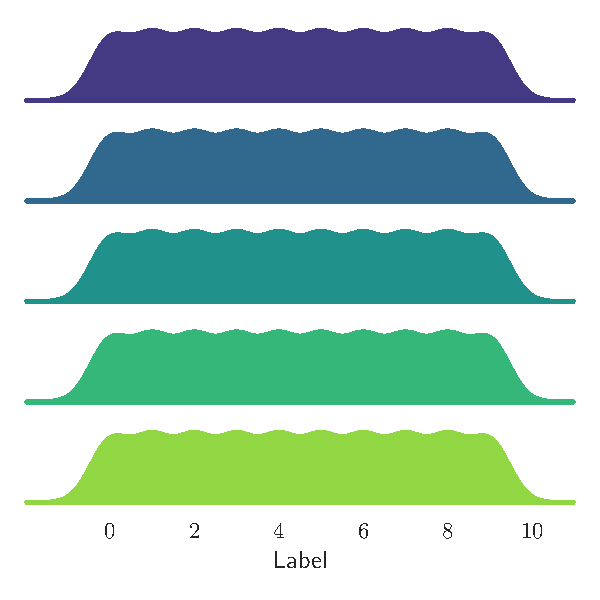
\includegraphics[width=\textwidth]{figures/ch07/lmcs/IID.pdf}
    \caption{IID partitioning.}
  \end{subfigure}
  \hfill
  \begin{subfigure}[b]{0.32\textwidth}
    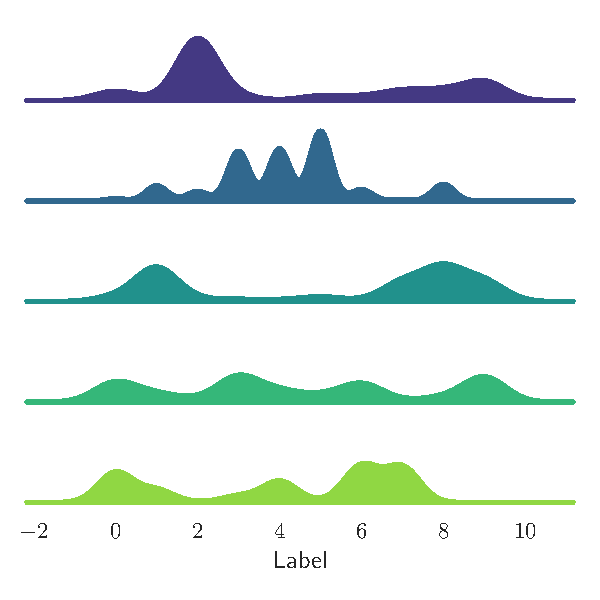
\includegraphics[width=\textwidth]{figures/ch07/lmcs/Dirichlet.pdf}
    \caption{Dirichlet partitioning.}
  \end{subfigure}
  \hfill
  \begin{subfigure}[b]{0.32\textwidth}
    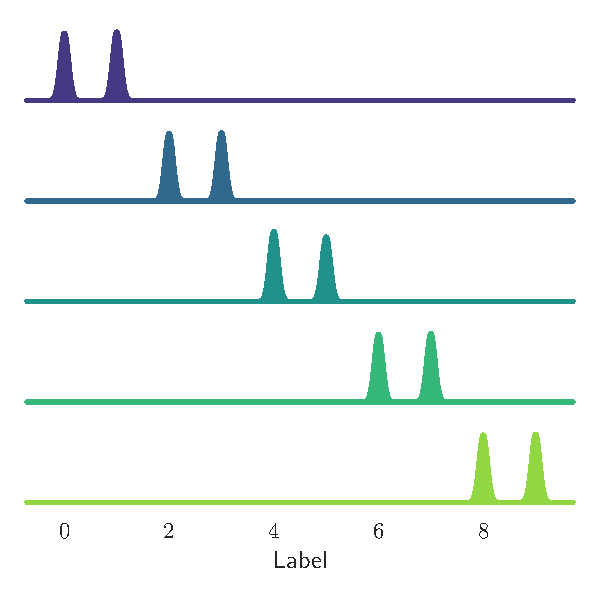
\includegraphics[width=\textwidth]{figures/ch07/lmcs/Hard.pdf}
    \caption{Hard partitioning.}
  \end{subfigure}
  \caption{The three data-partitioning modes of \textsc{ProFed}
    applied to MNIST with five subregions.
    Color saturation indicates the fraction of each class in each
    region.}
  \label{fig:profed-partitioning}
\end{figure}

\paragraph*{API Design.}
\textsc{ProFed} exposes a Python API that allows researchers to
 (i) download and cache the supported datasets,
 (ii) partition them into a configurable number of subregions with
 the desired skewness mode,
 and (iii) retrieve per-device dataset objects ready for
 integration with any \gls{FL} training loop~\cite{FBFL_cite09}.
%
The API is designed to require minimal configuration:
 a user specifies the dataset name, the number of subregions,
 and the partitioning mode,
 and receives device-indexed \texttt{Dataset} objects compatible
 with the standard PyTorch \texttt{DataLoader} interface.

\paragraph*{Quality Control.}
\textsc{ProFed} includes a validation suite that checks distributional
 properties of the generated splits (e.g., class-frequency balance
 within regions, inter-region divergence)
 and produces reproducible splits through seeded random number
 generation.
%
This allows experimental results to be exactly reproduced
 across different hardware and software environments.

\begin{figure}[htbp]
  \centering
  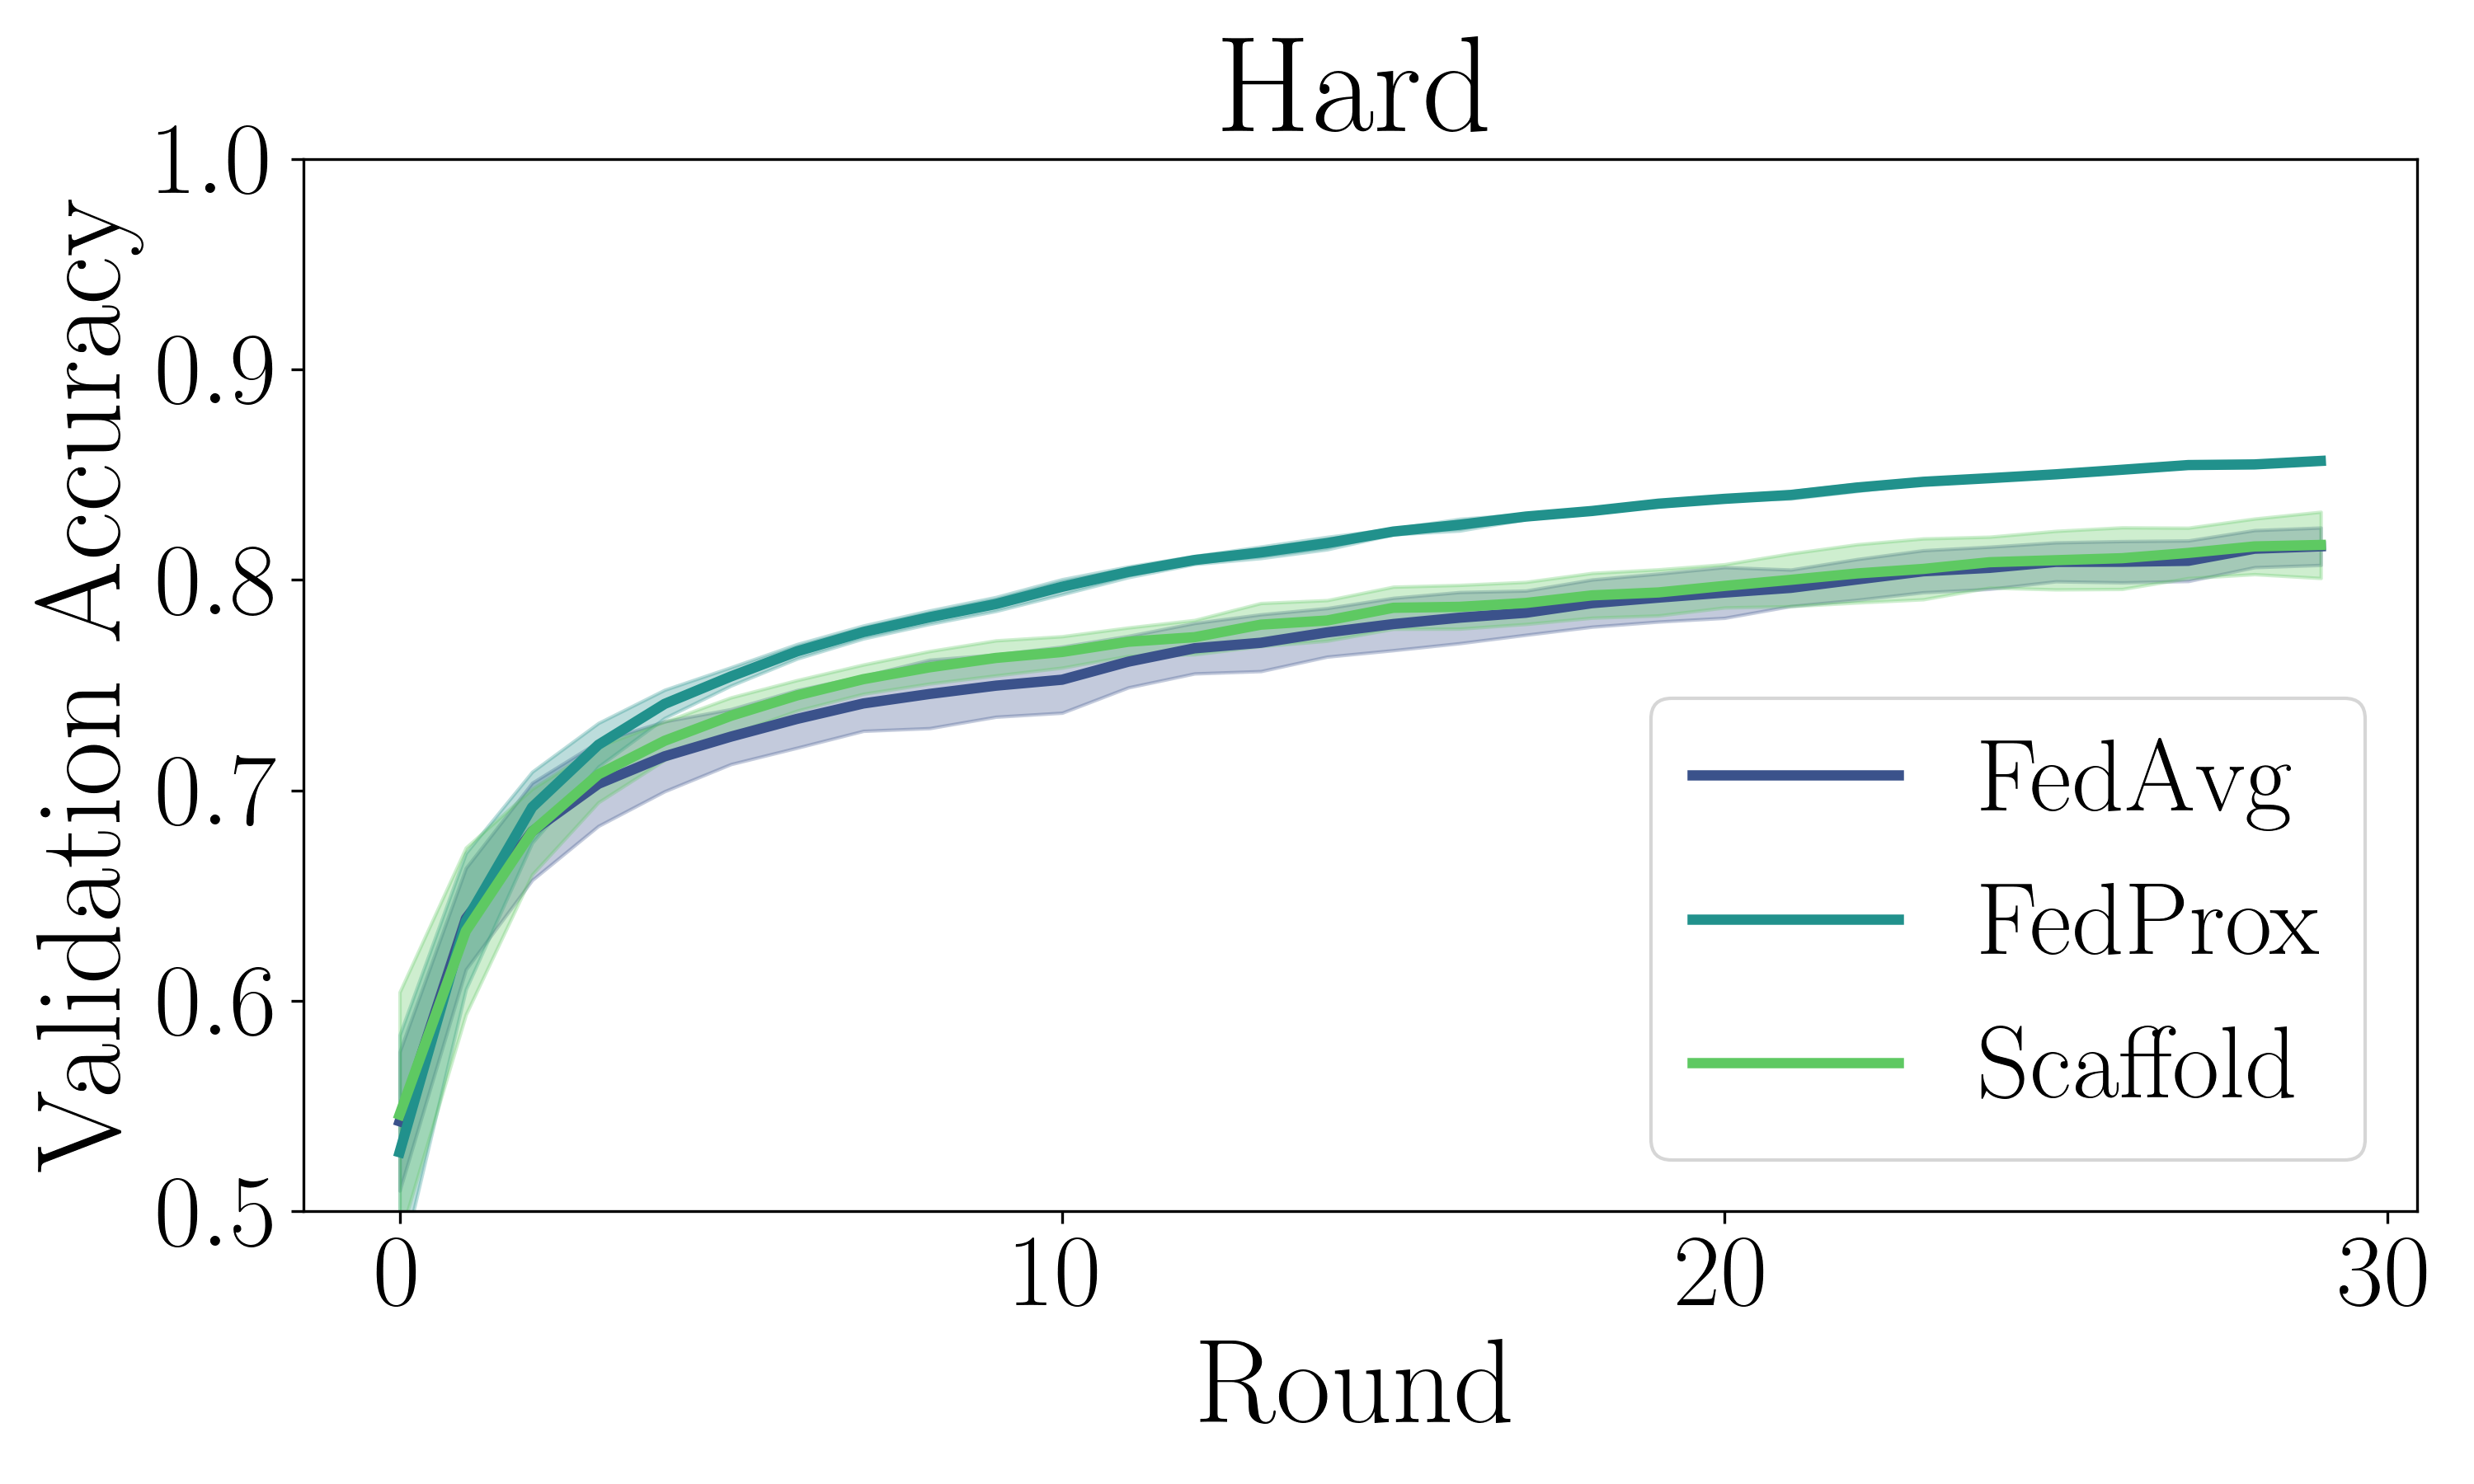
\includegraphics[width=0.8\textwidth]{figures/ch07/profed/charts/ValidationAccuracy_dataset-MNIST_areas-3_partitioning-Hard.png}
  \caption{Validation accuracy curves produced by \textsc{ProFed}
    on MNIST with 3 areas and Hard partitioning.
    Results for multiple \gls{FL} algorithms are plotted side by side
    for direct comparison.}
  \label{fig:profed-accuracy}
\end{figure}

The benchmark was used in all evaluation experiments reported in
 \Cref{subsec:fbfl,subsec:psfl,subsec:sparseful},
 ensuring consistent comparisons across algorithms and datasets.


%=============================================================================
\section{Related Work}
\label{sec:selforgfl-related}
%=============================================================================

The work presented in this chapter intersects three research lines:
 clustered \gls{FL}, decentralized \gls{FL},
 and field-based coordination.
%
The following situates the contributions with respect to the
 most closely related methods.

\paragraph*{Clustered Federated Learning.}
The problem of clustering clients to improve \gls{FL} under
 data heterogeneity has been addressed from several angles.
%
IFCA~\cite{FBFL_cite02} alternates between cluster assignment
 (each client evaluates all cluster models and picks the one with
 lowest local loss) and model update (each cluster model is
 aggregated from the clients assigned to it).
%
FeSEM~\cite{FBFL_cite03} formulates clustering as an expectation-maximization
 problem and iterates between E-step cluster assignment and M-step
 model aggregation.
%
Gradient-based methods~\cite{FBFL_cite04} cluster clients by comparing
 the cosine similarity of their gradient updates.
%
All of these approaches share two assumptions that the present work
 does not make: a central server performs the cluster assignment,
 and the number of clusters is provided as input.
%
The proposed methods operate fully decentralized and discover the
 number of federations automatically through the self-organizing
 coordination protocol.

Similarity measures for cluster formation have been studied in the
 federated setting along three main axes~\cite{FBFL_cite15}:
 loss-based (the approach adopted here),
 gradient-based, and weight-based.
%
Loss-based measures require cross-evaluation of neighbor models on
 the local dataset,
 which is privacy-preserving in the sense that only scalar loss values
 (and model parameters) are exchanged, not raw data.

\paragraph*{Decentralized Federated Learning.}
Gossip-based \gls{FL} algorithms~\cite{FBFL_cite16} replace the
 central server with peer-to-peer model averaging,
 achieving communication without coordination overhead.
%
Topology-aware variants~\cite{FBFL_cite17} weight the gossip steps
 by network connectivity to improve convergence.
%
These methods train a single global model and do not address
 the heterogeneity problem.
%
The present work combines decentralized coordination with clustered
 training, providing both the absence of a central server and the
 per-cluster specialization needed under non-\gls{IID} data.

\paragraph*{Field-Based Coordination.}
The \gls{SCR} pattern~\cite{FBFL_cite08} was originally developed for
 generic self-organization in spatial computing,
 with applications to sensor networks and robot swarms.
%
Its application to \gls{FL} was novel at the time of the
 \gls{FBFL} publication~\cite{FBFL_cite05}.
%
Space-fluid computing~\cite{FBFL_cite18} extends the aggregate
 computing model with metric spaces that need not be physical,
 and the present work instantiates this abstraction through the
 model-dissimilarity metric in \gls{PSFL}.

\paragraph*{Neural Network Sparsification.}
Unstructured magnitude-based pruning~\cite{FBFL_cite19} is a
 well-established technique for reducing model size,
 and it has been studied in the federated setting mainly as a
 way to reduce communication volume~\cite{FBFL_cite20}.
%
\textsc{SParSeFuL} is distinctive in that sparsification actively
 shapes the federation topology: the sparse models are used as
 the dissimilarity signals that drive region formation,
 creating a feedback loop between model compression and cluster
 structure that, to the best of our knowledge, has not been
 explored before.


%=============================================================================
\section{Future Directions}
\label{sec:selforgfl-future}
%=============================================================================

The contributions described in the preceding sections assume that
 the device population is static and that the data distribution at each
 device does not change over time.
%
Two ongoing research threads relax these assumptions.

\subsection{C\textsuperscript{2}FL: Continual Clustered Federated Learning for Moving Nodes}
\label{subsec:c2fl}

In many \gls{CAS} scenarios---vehicular networks, robot fleets,
 wearable devices---nodes move through an environment that exhibits
 spatial data heterogeneity.
%
When a device crosses from one data region into another,
 the distribution of its locally observed data changes abruptly,
 inducing a \emph{sequential distribution shift}.
%
Training on the new distribution without precaution degrades
 performance on previously learned distributions,
 a phenomenon known as \emph{catastrophic forgetting}~\cite{FBFL_cite21}.

\textsc{C$^2$FL}~\cite{FBFL_cite22} (Clustered Continual Federated Learning)
 addresses this challenge by combining the self-organizing clustering
 protocol with two \gls{CL} mechanisms:
 \emph{experience replay} and \emph{adaptive averaging}.

\paragraph*{Mobility-Induced Task Stream.}
Each device $d$ accumulates a sequence of tasks
 $\mathcal{T}_d^{(1)}, \mathcal{T}_d^{(2)}, \ldots$
 as it transitions through different spatial regions.
%
The task history up to round $t$ is
 $\mathcal{H}_d^{(t)} = \{\mathcal{T}_d^{(1)}, \ldots, \mathcal{T}_d^{(t)}\}$.
%
A region transition is detected when the assigned leader changes:
 $\eta_d^{(t)} \ne \eta_d^{(t-1)}$.
%
Upon transition, the device's local dataset from the previous region
 is added to a replay memory $\mathcal{M}_d^{(t)}$,
 and a permanence counter $s_d^{(t)}$ resets to 1.
%
During subsequent rounds within the new region, $s_d^{(t)}$ increments
 by 1 per round.

\paragraph*{Experience Replay.}
During local training the device interleaves samples from the
 current dataset $\mathcal{D}_d^{(t)}$ with samples from
 $\mathcal{M}_d^{(t)}$,
 preserving knowledge accumulated in previously visited regions
 without requiring access to past data beyond what is stored in memory.
%
The replay memory is never shared with other devices,
 so it does not introduce new privacy risks.

\paragraph*{Adaptive Averaging.}
After aggregation the leader broadcasts the regional model
 $\theta_k^{(t+1)}$ to region members.
%
The device merges this regional model into its local state through
 a dwell-time-aware mixing rule.
%
The mixing factor $\alpha_d^{(t)}$ grows with permanence in the
 current region:
\begin{equation}
  \alpha_d^{(t)} = \min\!\left\{\Gamma,\; \frac{s_d^{(t)}}{H}\right\},
  \label{eq:c2fl-mixing}
\end{equation}
where $\Gamma \in [0,1]$ is the maximum mixing factor
 and $H > 0$ is an adaptation horizon.
%
The final device model is:
\begin{equation}
  \theta_d^{(t+1)}
    = \bigl(1 - \alpha_d^{(t)}\bigr)\,\tilde{\theta}_d^{(t+1)}
    + \alpha_d^{(t)}\,\theta_k^{(t+1)},
  \label{eq:c2fl-update}
\end{equation}
where $\tilde{\theta}_d^{(t+1)}$ is the model after local training
 with replay.
%
Immediately after a region transition the mixing factor is small,
 giving priority to local adaptation;
 as permanence increases, the contribution of the regional consensus
 grows, progressively aligning the device with its new cluster.

\begin{figure}[htbp]
  \centering
  \begin{subfigure}[b]{0.48\textwidth}
    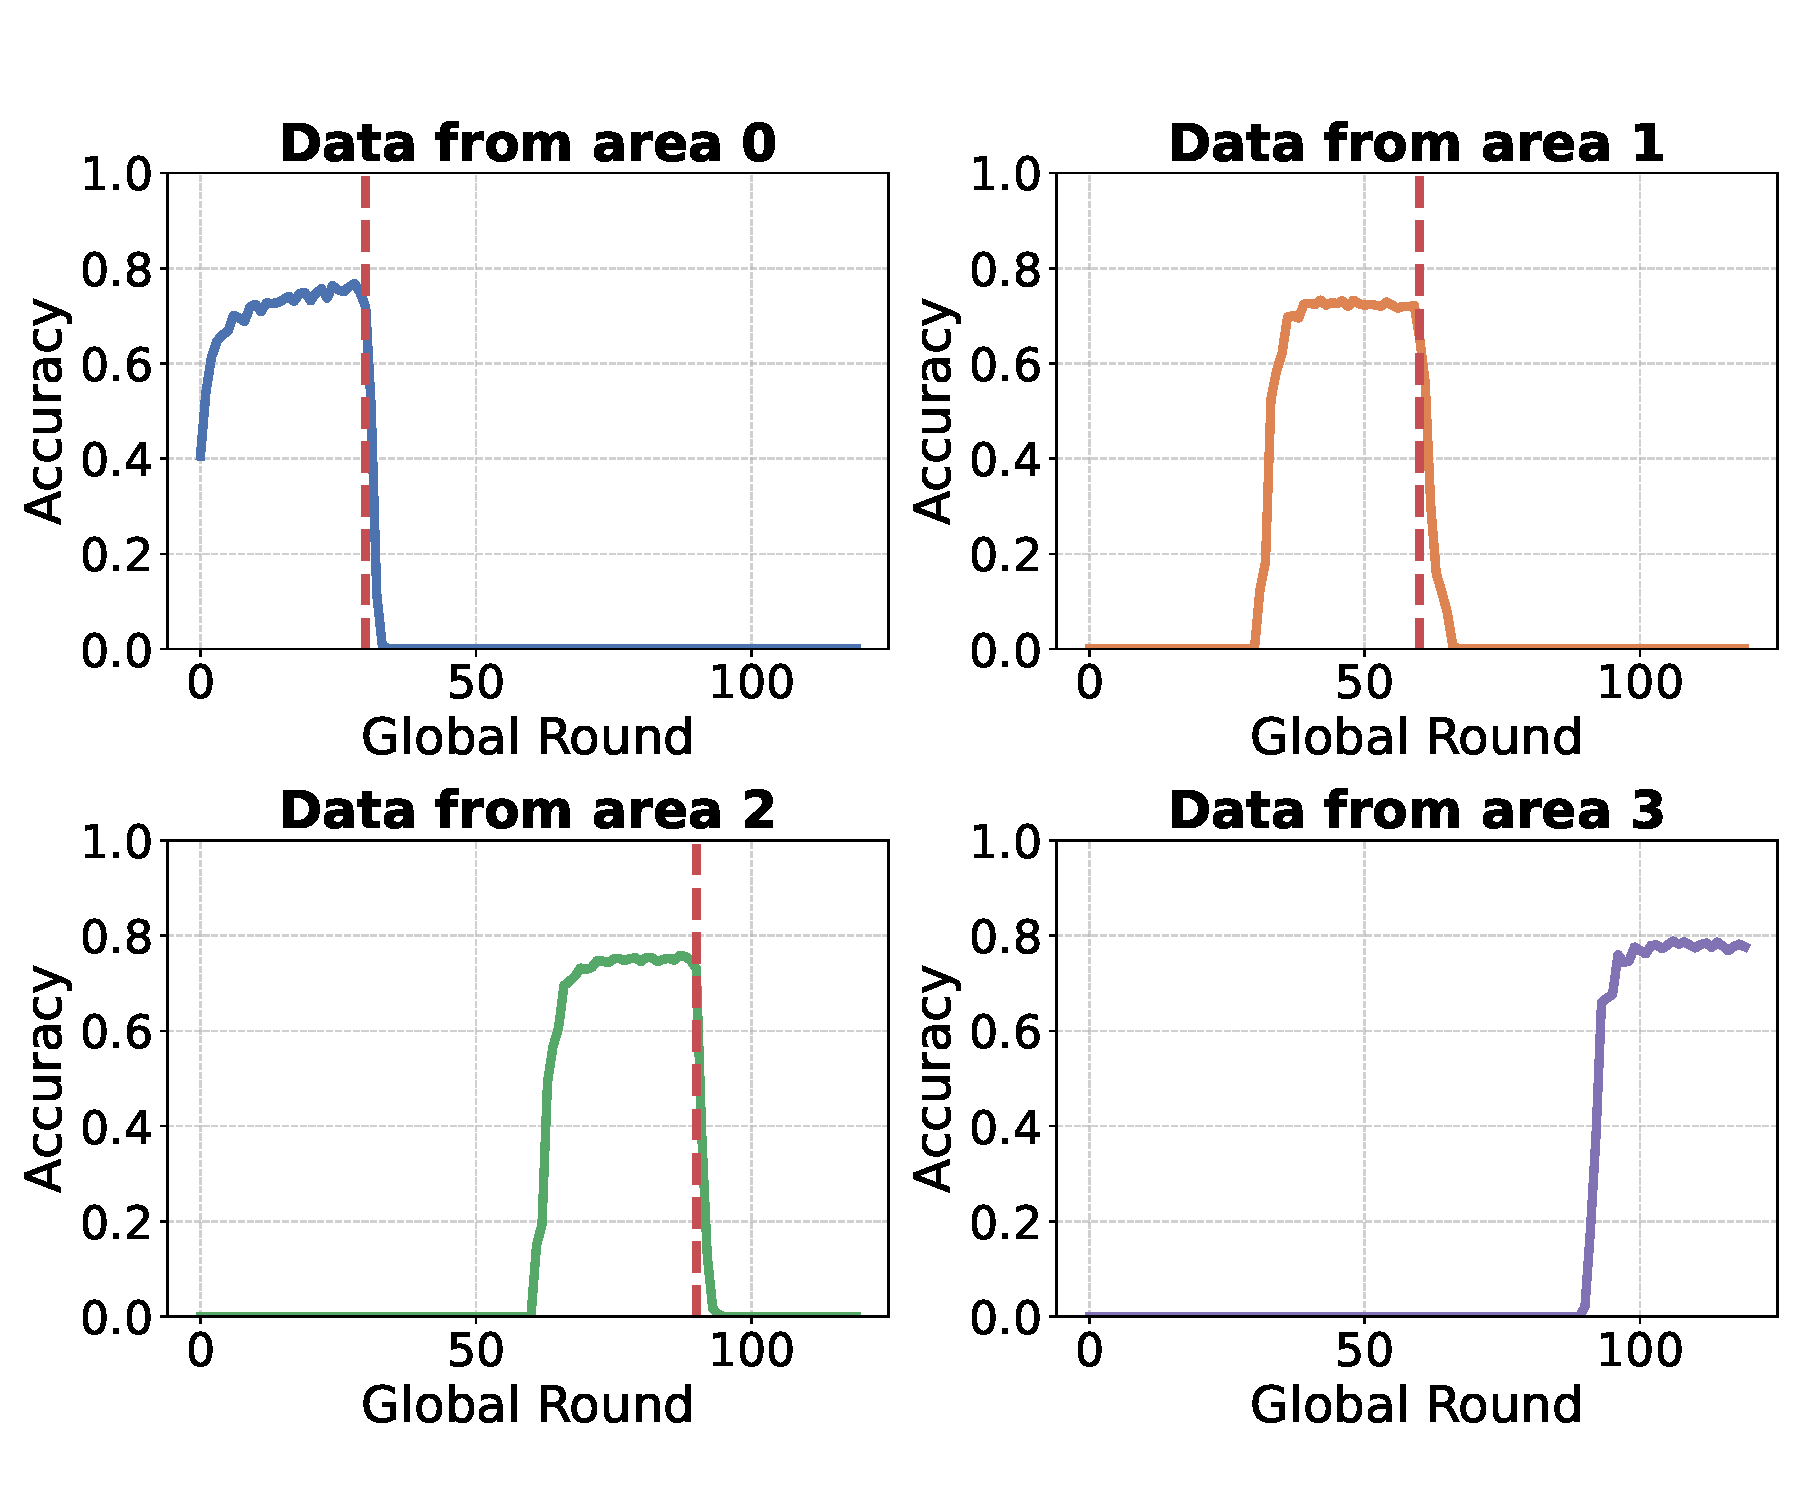
\includegraphics[width=\textwidth]{figures/ch07/c2fl/moving-node-FL_merge.pdf}
    \caption{Standard \gls{FL}: catastrophic forgetting during node
      movement.}
  \end{subfigure}
  \hfill
  \begin{subfigure}[b]{0.48\textwidth}
    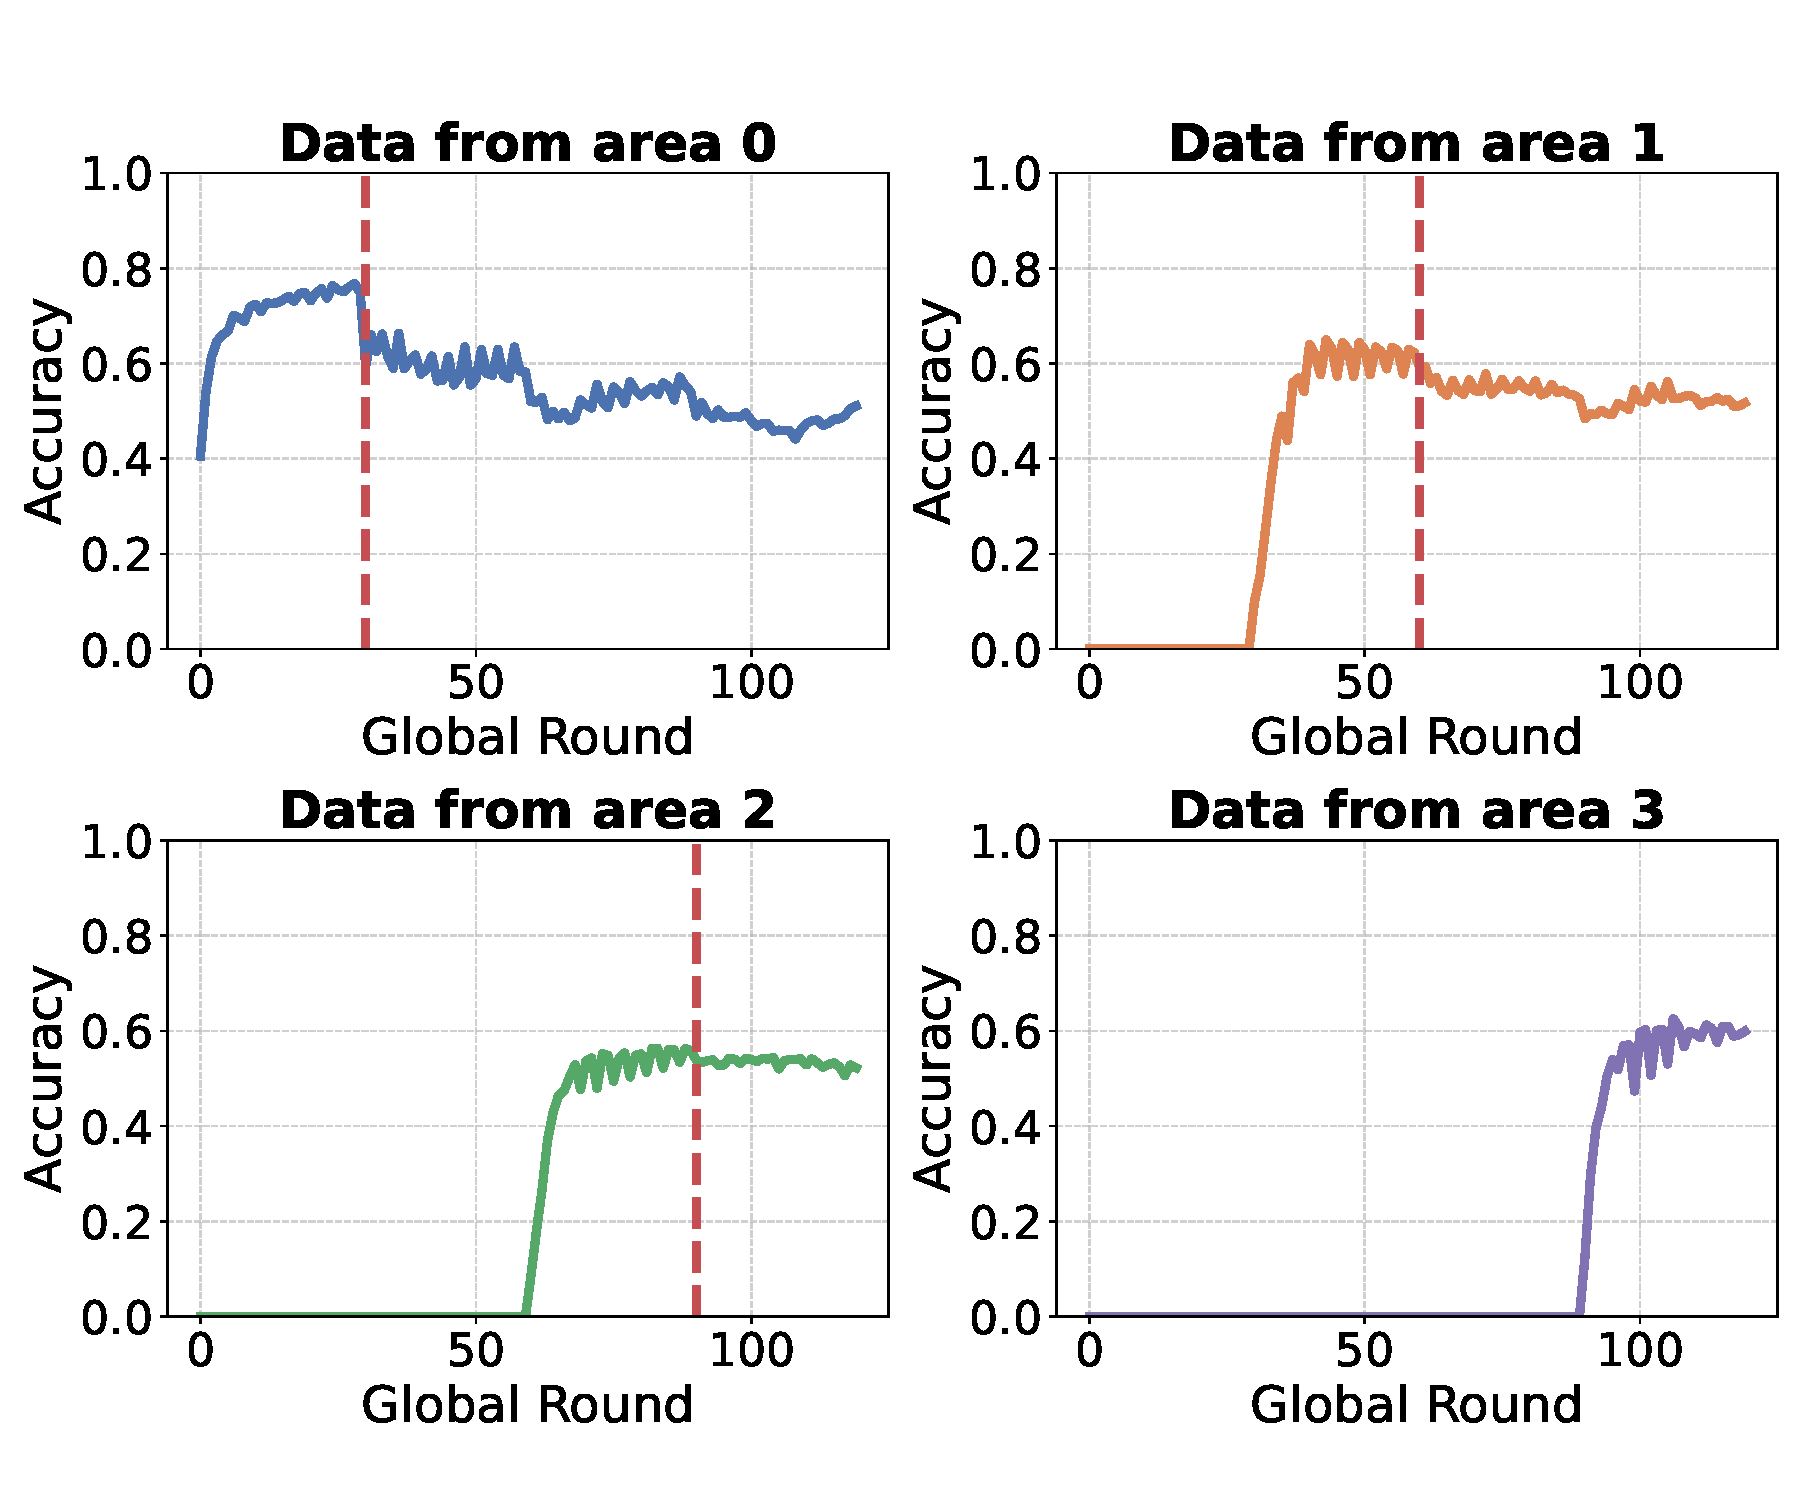
\includegraphics[width=\textwidth]{figures/ch07/c2fl/moving-node-C2FL_merge.pdf}
    \caption{\textsc{C$^2$FL}: controlled adaptation with replay and
      adaptive averaging.}
  \end{subfigure}
  \caption{Effect of node movement on model performance.
    Standard clustered \gls{FL} degrades performance on previously
    learned regions;
    \textsc{C$^2$FL} mitigates forgetting through replay and
    dwell-time-aware mixing.}
  \label{fig:c2fl-comparison}
\end{figure}

\begin{figure}[htbp]
  \centering
  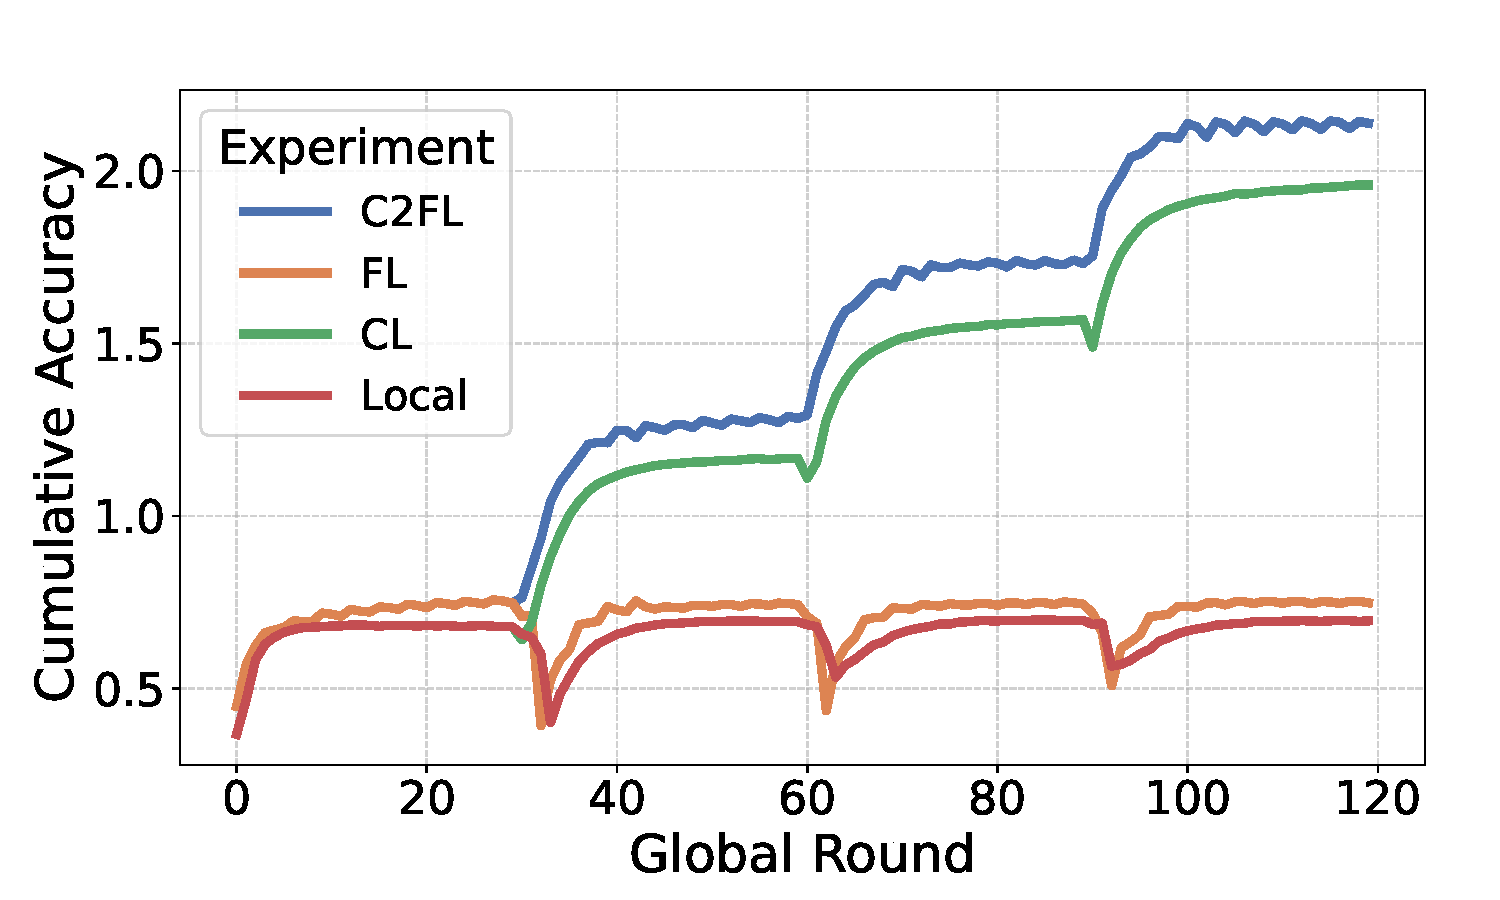
\includegraphics[width=0.75\textwidth]{figures/ch07/c2fl/comparison.pdf}
  \caption{Cumulative accuracy comparison between \textsc{C$^2$FL}
    and baselines under node mobility.
    \textsc{C$^2$FL} achieves higher retention of past-region knowledge
    while adapting to new distributions.}
  \label{fig:c2fl-cumulative}
\end{figure}

Preliminary results confirm that mobility-induced distribution shifts
 cause significant forgetting in standard clustered \gls{FL},
 and that the combination of replay and adaptive averaging substantially
 reduces this effect while preserving adaptation speed to the
 current region~\cite{FBFL_cite22}.


\subsection{Uncertainty-Based Clustering with Random Network Distillation}
\label{subsec:rnd}

The clustering mechanisms in \gls{FBFL} and \gls{PSFL} rely on
 loss-based dissimilarity, which requires each device to evaluate
 all neighbor models on its local dataset at every federation-formation step.
%
While this cost is local (scaling with the neighborhood size rather
 than the total population),
 it still requires sharing full model parameters with neighbors
 and performing forward passes on the local validation set.
%
A lighter alternative is to use \emph{uncertainty estimates} as
 a proxy for distributional divergence,
 avoiding the need to exchange task models for clustering purposes.

The second extension~\cite{FBFL_cite23} applies \gls{RND}~\cite{FBFL_cite24}
 to this problem.
%
\gls{RND} was originally introduced in the \gls{RL} literature
 as a measure of epistemic uncertainty,
 but its core mechanism---training a small predictor network to
 mimic a fixed random target---produces uncertainty estimates that
 are high on inputs outside the training distribution,
 making it a natural fit for cluster discovery.

\paragraph*{RND Predictor Training.}
Each device $d_i$ trains a compact \gls{RND} predictor
 $\hat{f}_i(\cdot;\theta_i)$ by minimizing the expected
 squared prediction error with respect to a shared,
 randomly initialized target network $f$:
\begin{equation}
  \theta_i^* = \arg\min_{\theta}
    \mathbb{E}_{x \sim \mathcal{B}_i}
    \bigl\| \hat{f}_i(x;\theta) - f(x) \bigr\|_2^2,
  \label{eq:rnd-training}
\end{equation}
where $\mathcal{B}_i$ is a mini-batch of local data.
%
Once trained, the predictor $\hat{f}_i(\cdot;\theta_i^*)$ generalizes
 well to inputs from the same distribution as $\mathcal{B}_i$
 and produces high residuals on inputs from different distributions.

\paragraph*{Cross-Novelty Matrix.}
Each device broadcasts its trained predictor to all other devices.
%
Device $d_i$ evaluates every received predictor $\hat{f}_j$
 on its own local data batch,
 computing a cross-novelty score:
\begin{equation}
  s_{ij} = \mathbb{E}_{x \sim \mathcal{B}_i}
    \Bigl\| \hat{f}_j(x;\theta_j^*) - f(x) \Bigr\|_2^2,
  \qquad \forall j \in \{1, \ldots, N\}.
  \label{eq:rnd-crossnovelty}
\end{equation}
%
Low $s_{ij}$ means that $\hat{f}_j$ generalizes well to $d_i$'s data,
 implying similar distributions;
 high $s_{ij}$ signals distributional divergence.
%
The scores $\{s_{ij}\}_{j=1}^N$ are reported to a server,
 which reconstructs the full cross-novelty matrix
 $S \in \mathbb{R}^{N \times N}$
 without accessing any raw data.

\begin{figure}[htbp]
  \centering
  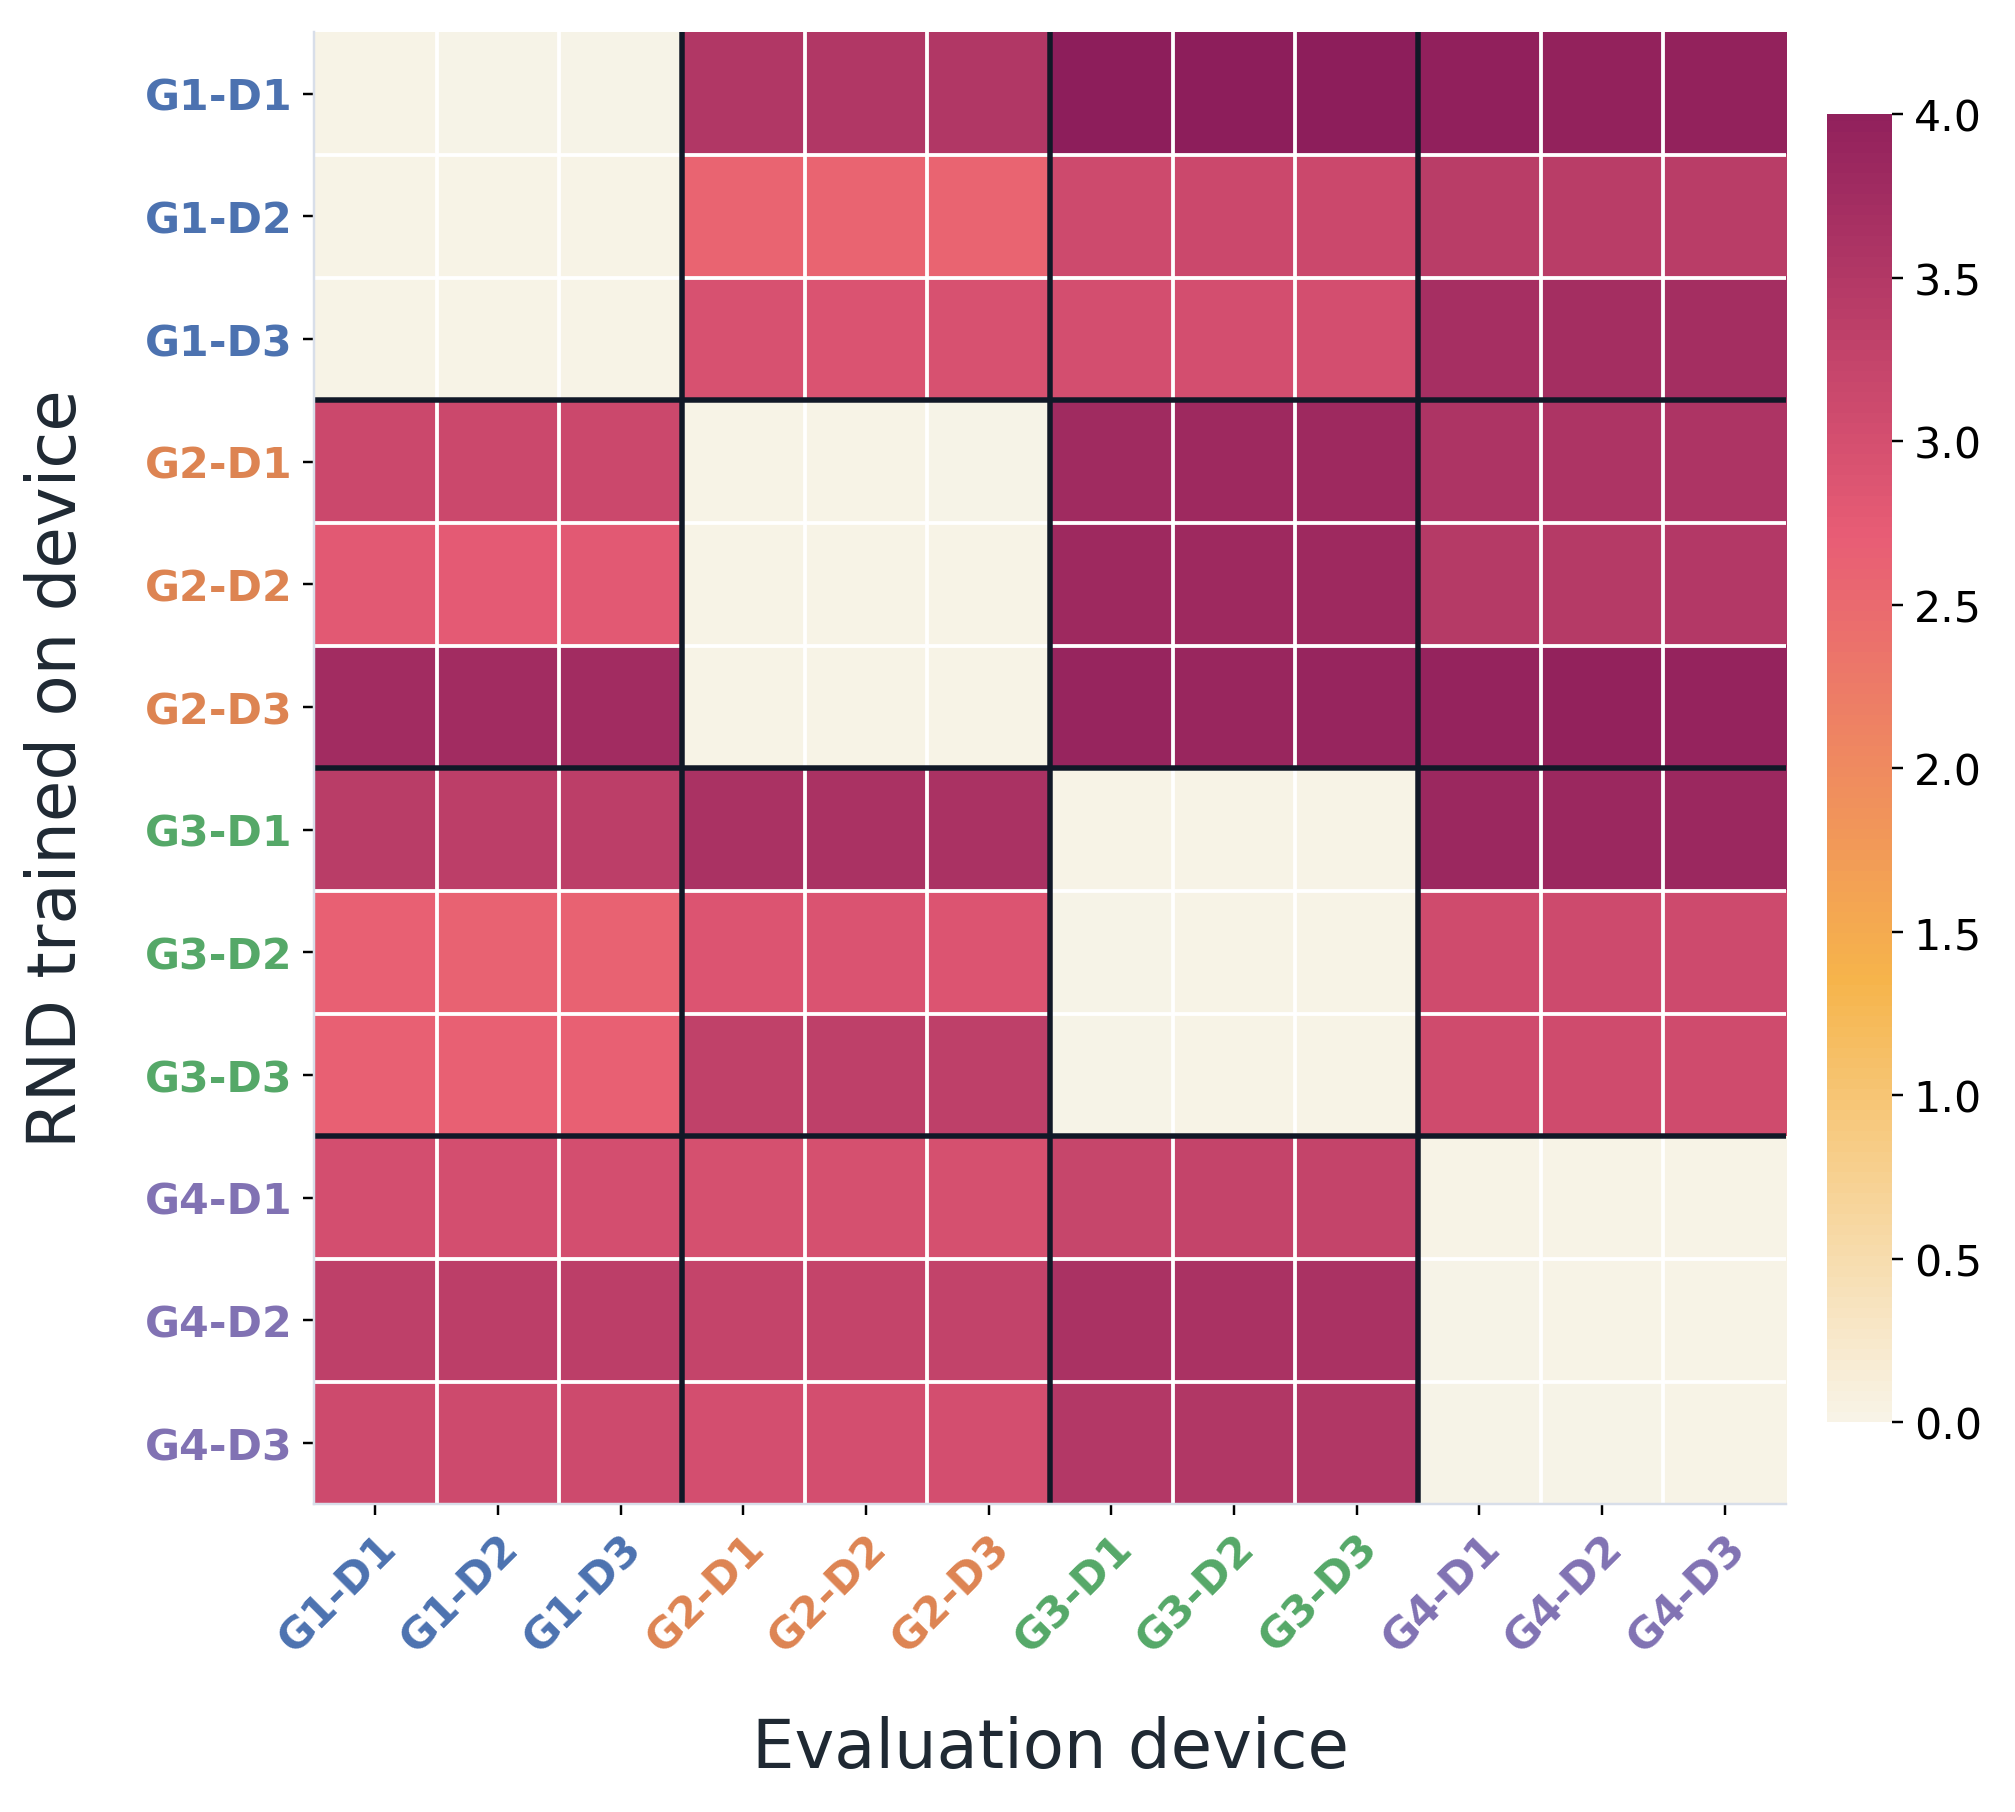
\includegraphics[width=0.75\textwidth]{figures/ch07/rnd/uncertainty_difference_heatmap.png}
  \caption{Difference between self-novelty $s_{ii}$ and cross-novelty
    $s_{ij}$ across devices.
    Devices within the same ground-truth cluster show low cross-novelty
    relative to self-novelty;
    inter-cluster pairs show high cross-novelty,
    confirming that \gls{RND} residuals expose the latent cluster
    structure without raw data exchange.}
  \label{fig:rnd-heatmap}
\end{figure}

\paragraph*{Adaptive Federation Discovery.}
Rather than specifying the number of clusters in advance,
 the partition is derived from the compatibility criterion:
 device $d_j$ is compatible with $d_i$ if
\begin{equation}
  s_{ij} \le s_{ii} + \epsilon \cdot \sigma_i,
  \label{eq:rnd-compatibility}
\end{equation}
where $s_{ii}$ is the self-novelty of $d_i$ (the residual error on
 its own data),
 $\sigma_i$ is the standard deviation of $\{s_{ij}\}_{j=1}^N$,
 and $\epsilon \ge 0$ is a tolerance hyperparameter.
%
The number of federations emerges as the number of distinct
 compatibility groups,
 expected to converge to the true number of clusters $K$~\cite{FBFL_cite23}.

\begin{figure}[htbp]
  \centering
  \begin{subfigure}[b]{0.48\textwidth}
    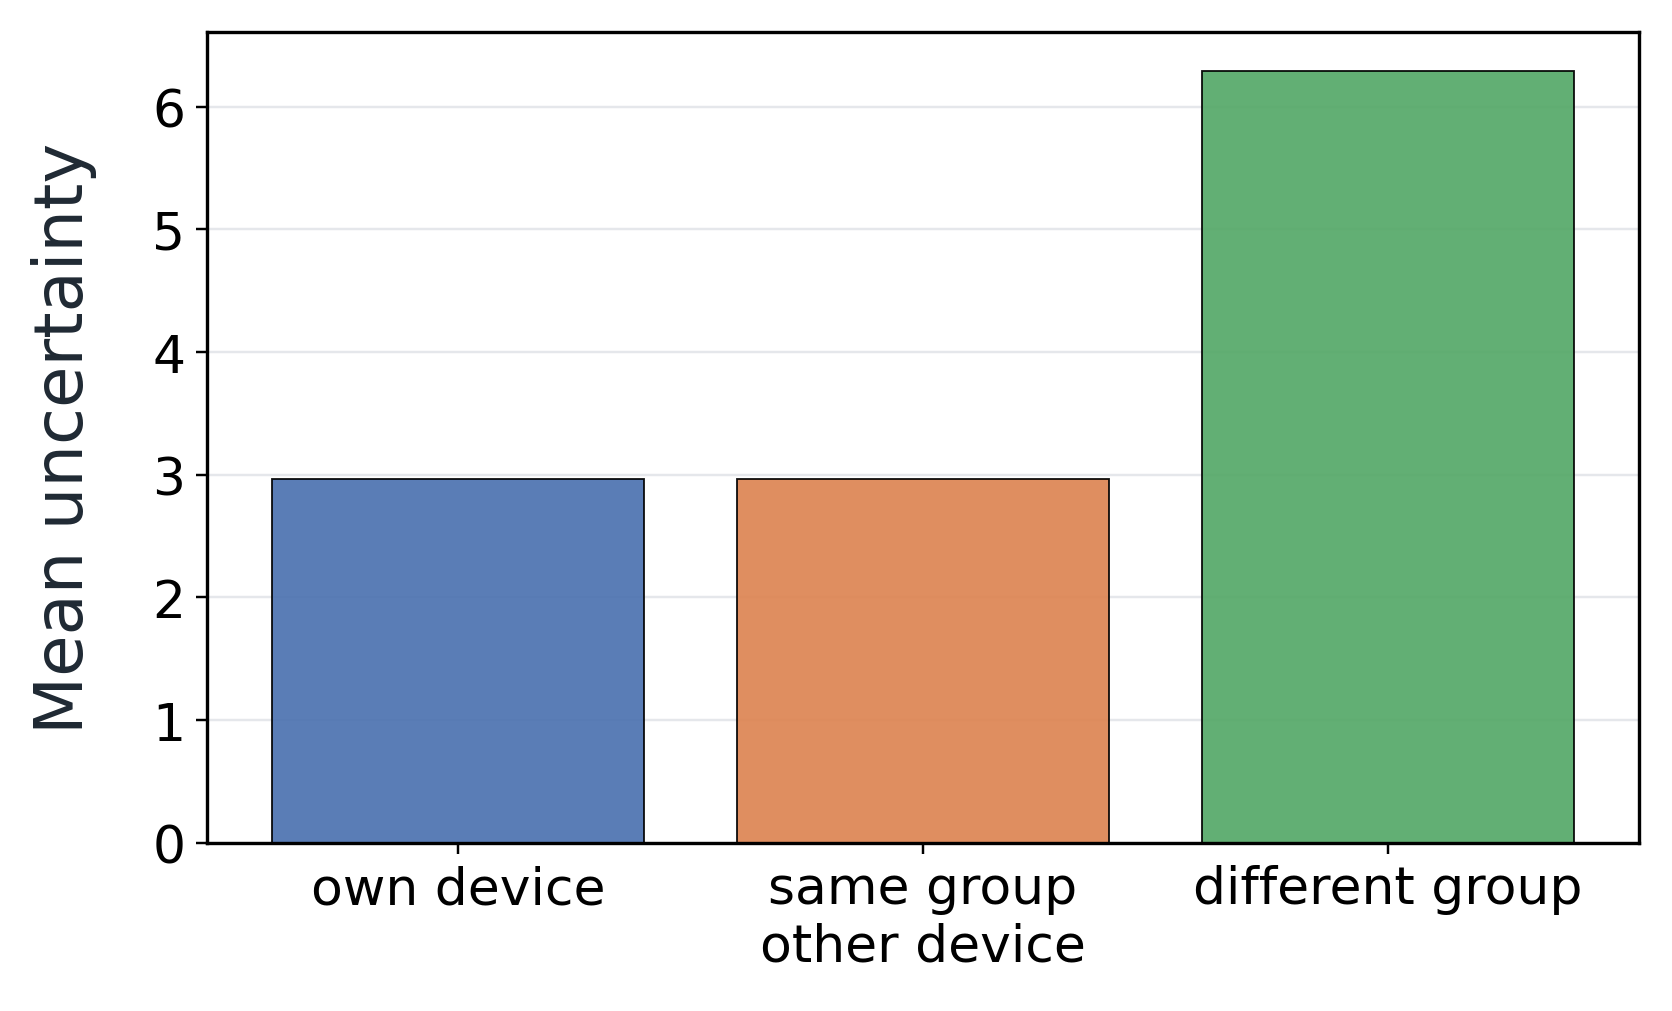
\includegraphics[width=\textwidth]{figures/ch07/rnd/diagonal_vs_offdiagonal_barplot.png}
    \caption{Self-novelty vs.\ cross-novelty across cluster pairs.}
  \end{subfigure}
  \hfill
  \begin{subfigure}[b]{0.48\textwidth}
    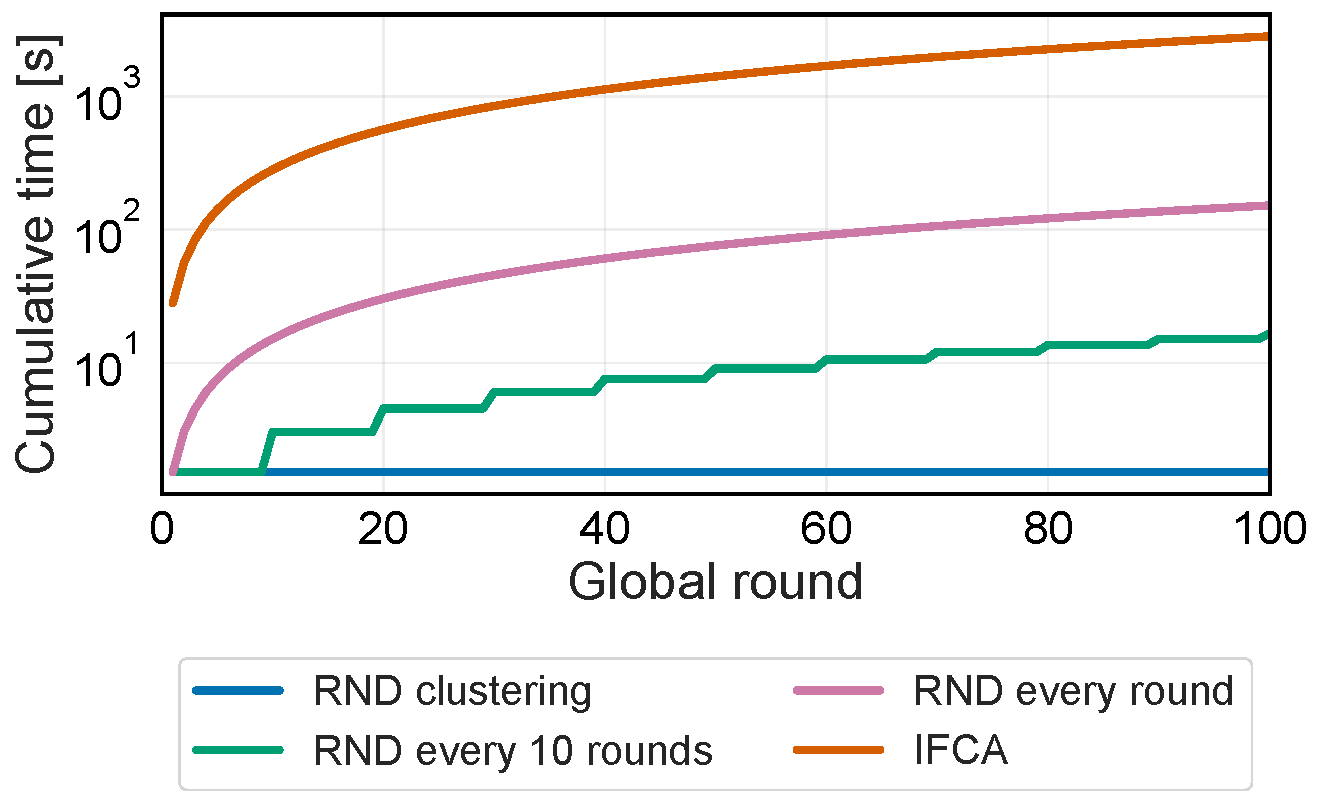
\includegraphics[width=\textwidth]{figures/ch07/rnd/cumulative_time.pdf}
    \caption{Cumulative clustering time vs.\ IFCA.}
  \end{subfigure}
  \caption{RND-based clustering results.
    The diagonal vs.\ off-diagonal difference confirms distributional
    separability;
    clustering cost is substantially lower than IFCA because
    re-clustering is needed only when distributions shift,
    not at every round.}
  \label{fig:rnd-results}
\end{figure}

\paragraph*{Clustering Frequency.}
In stationary environments the clustering phase is performed once,
 prior to any federated training round,
 since the cluster structure is not expected to change.
%
In non-stationary environments the procedure can be re-triggered
 periodically with interval $\tau$ (measured in federated rounds),
 allowing the system to adapt to distributional drift.
%
Setting $\tau = +\infty$ recovers the stationary case;
 small values of $\tau$ enable continuous adaptation at increased cost~\cite{FBFL_cite23}.

Preliminary results show that \gls{RND} uncertainty estimates
 effectively separate devices from different ground-truth clusters
 without requiring task-model sharing,
 and that the compatibility criterion discovers the correct number
 of federations under the tested configurations.
%
The computational cost of the \gls{RND} clustering phase is
 substantially lower than IFCA's re-evaluation-based assignment,
 particularly when re-clustering is triggered infrequently~\cite{FBFL_cite23}.

